\chapter{Trends: How different factors affect the grating efficiency}
With new software tools in-hand, we move on to the next question: What can we learn from them about the efficiency of gratings, especially those used in typical soft x-ray instruments?

This chapter looks at the theoretical effects caused by changes to grating parameters: groove profile, shape (depth, duty cycle, angles, etc.), line density, coating material, coating thickness, and incidence angle.  We can think of the grating efficiency as a scalar function of this many-dimensional parameter space, but it is impossible to capture its complexity in a simple analytical equation.  None the less, the results in this chapter should give beamline designers an understanding of trends along each dimension within this space, and how to apply these trends to the optimization of gratings.

We attempt to isolate the effects of each parameter as much as possible.  However, many parameters are linked together so that they cannot be made independent.  For example, as we show in Section \ref{blazeAngle}, gratings with triangular profiles have an optimal \emph{blaze angle} (the angle at the base of the light-facing facet, Figure \ref{3d}) that aligns the outgoing diffraction order with the specular reflection for maximum efficiency.  For this type of grating, changing only the groove density will change the outgoing diffraction angle, and therefore change the optimal blaze angle.  Simply plotting the efficiency as a function of groove density while holding all other parameters constant would confuse the blaze effect with the density effect; instead, we correct for this by adjusting the angle to keep the grating ``on-blaze'' as we vary the groove density in Figure \ref{3e}.

All of the calculations in this chapter were computed with the differential method, using either \texttt{\textbf{Gradif}} or our new \texttt{\textbf{PEG}} implementation.  Unless otherwise noted, results are shown for randomly polarized (natural) light, which is an average of the TM and TE efficiency.  When we refer to 1st and 2nd order efficiencies without clarification, we implicitly mean the inside orders ($n<0$).\footnote{At grazing incidence, the outside orders are usually suppressed completely, since they would end up inside the grating. In the Rayleigh expansion \eq{rayleighExp2}, they end up as evanescent (decaying) rather than propagating orders.}
\section{Effect of grating profile: groove shape}

As we showed in Chapter 3, any kind of periodic groove structure will have a diffraction effect, regardless of the nature of the groove shape.  However, the grating efficiency -- particularly in the order the experimenter wants to use -- depends substantially on the groove shape.  

Five common groove profiles are shown in Figure \ref{3c-profile}: a classic rectangular profile, a triangular profile (also known as a ``sawtooth'' or ``blazed'' pattern), a trapezoidal profile, a sinusoidal profile, and an approximated triangular profile.

\begin{figure}[htbp] %  figure placement: here, top, bottom, or page
   \centering
   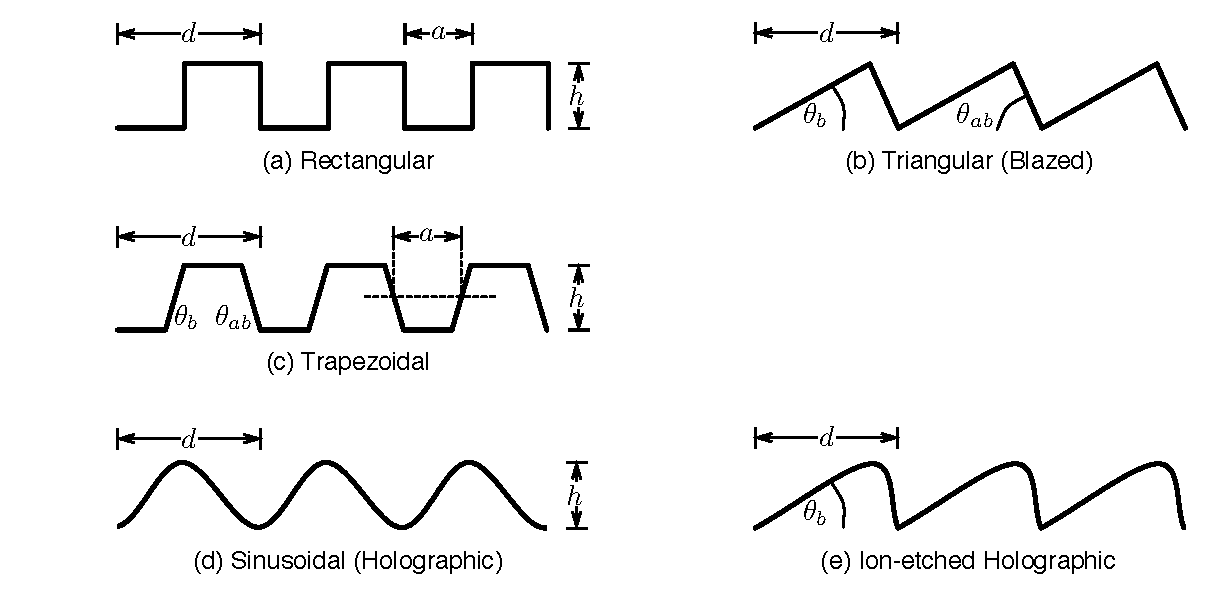
\includegraphics[width=\textwidth]{Chapter3/3c_effectOfProfile/3c_profiles.pdf}
   \caption[5 common groove profiles and their geometry parameters.]{5 common groove profiles and their geometry parameters.  The rectangular profile (a) and triangular profile (b) are idealized versions of those produced by mechanical ruling.  The trapezoidal profile (c) is usually produced accidentally while trying to rule a rectangular profile with an imperfect ruling tip.  The sinusoidal profile (d) is the natural shape produced by holographic ruling; the result can be ion-etched to approximate a triangular profile (e).}
   \label{3c-profile}
\end{figure}

\subsection{Note on grating manufacturing techniques}
\label{gratingManufacturing}
These types of profiles emerged largely as a consequence of grating manufacturing techniques.  To understand the impact of manufacturing on groove shape, we take a look at two techniques for creating gratings: mechanical and holographic ruling.

\noindent \textbf{\emph{Mechanical Ruling}}

\noindent In 1880, Henry Rowland invented a method for machining long, precise screws \cite{Row02}, and this enabled him to create a ``ruling engine'' (Figure \ref{3c-rowlandEngine}) for mechanically scratching fine parallel lines into a layer of metal on a substrate material.  His version was much more accurate than previous machines because it self-compensated for systematic errors in the screw pitch, and his efficient production of high-quality gratings ``revolutionized spectroscopy'' \cite{Wea76}.  Today, there are several extremely precise ruling engines around the world, using diamond tips and interferometric position feedback to mechanically engrave groove densities approaching 3~000 lines/mm.\footnote{The Michelson ruling engine, now owned by the Newport Corporation, can rule up to an astonishing 10~800 lines/mm.}

The rectangular and triangular profiles in Figure \ref{3c-profile} are a consequence of the shape of mechanical ruling tips.  The trapezoidal profile is often produced accidentally when attempting to rule a rectangular profile with a non-ideal tip, as was the case for the gratings shown in Figures \ref{3j-3} and \ref{3j-4}.

%\begin{figure}[htbp] %  figure placement: here, top, bottom, or page
%   \centering
%   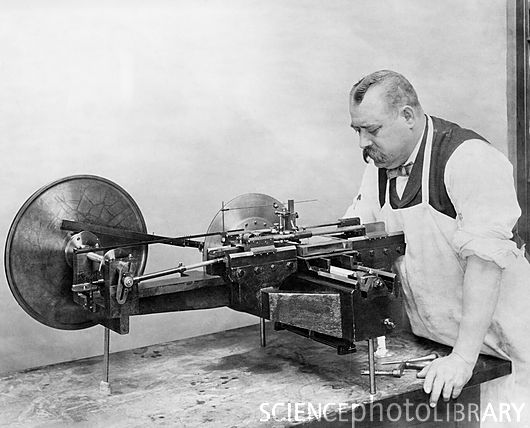
\includegraphics[width=0.8\textwidth]{Chapter3/3c_effectOfProfile/rowlandRulingEngine.jpg}
%   \caption[Henry Rowland's ruling engine, mechanically engraving a grating under the operation of his instrument maker Theodore Schneider.]{Henry Rowland's ruling engine, mechanically engraving a grating under the operation of his instrument maker Theodore Schneider.  Photographed at Johns Hopkins University, Baltimore.  \textbf{Image credit: }\textsc{Emilio Segre Visual Archives/American Institute Of Physics/Science Photo Library} (ref http://www.sciencephoto.com/media/150151/enlarge)}
%   \label{3c-rowlandEngine}
%\end{figure}
\begin{figure}[htbp] %  figure placement: here, top, bottom, or page
   \centering
   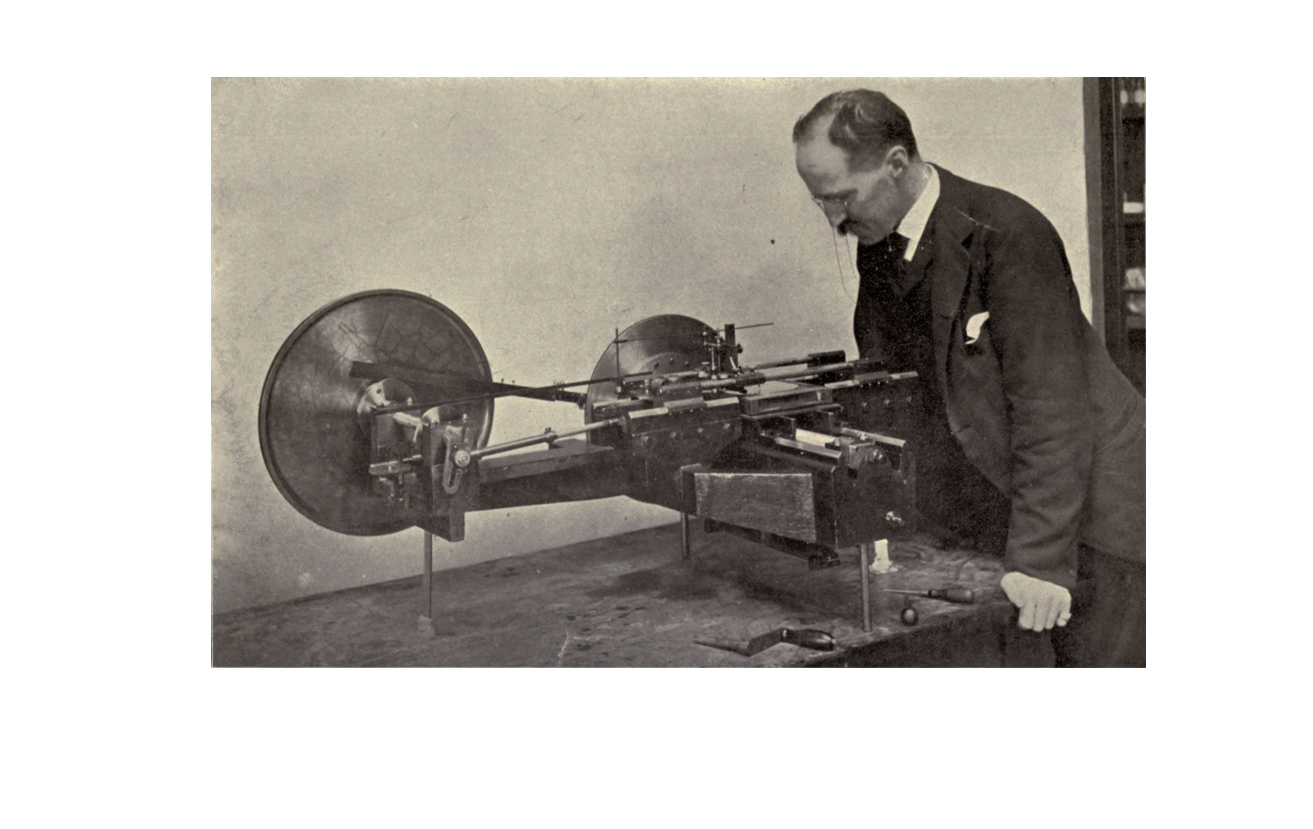
\includegraphics[width=0.8\textwidth]{Chapter3/3c_effectOfProfile/rowlandRulingEngine2_lowRes.pdf}
   \caption[Henry Rowland, supervising his mechanical engine ruling a grating.]{Henry Rowland, supervising his mechanical ruling engine ruling a grating.  Photographed at Johns Hopkins University, Baltimore.  Reprinted from \textsc{The Physical Papers of Henry Augustus Rowland} \cite[page 715]{Row02}}
   \label{3c-rowlandEngine}
\end{figure}

\begin{figure}[htbp] %  figure placement: here, top, bottom, or page
   \centering
   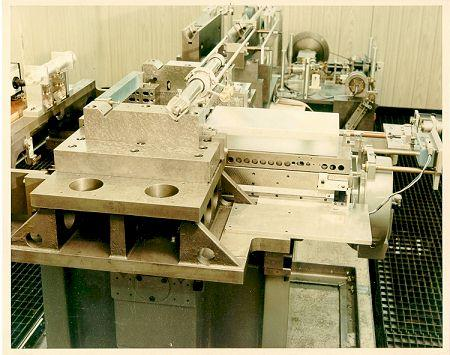
\includegraphics[width=\textwidth]{Chapter3/3c_effectOfProfile/mitBRulingEngine.jpg}
   \caption[The MIT `B' ruling engine, now owned and operated by Richardson Gratings (a division of the Newport Corporation).]{The MIT `B' ruling engine, now owned and operated by Richardson Gratings (a division of the Newport Corporation).  It can rule gratings up to 420 mm wide, with grooves up to 320 mm long.  The maximum groove density is 1500 lines/mm.  Equipped with a servo system for advancing the grating carriage and interferometric feedback using frequency-stabilized lasers, it is the most accurate ruling engine in the world.  To control for thermal expansion of the engine, the room temperature is controlled to 0.005$\deg$C; the system even compensates for changes in room air pressure since a change of just 2.5 mm of mercury will affect the refractive index of air (and therefore the interferometer wavelength) by one part per million.  The entire engine is suspended from springs to dampen vibrations between 3Hz to 60Hz, which could otherwise be transmitted to the diamond tip.  Reprinted from \textsc{The Diffraction Grating Handbook} \cite{Pal05}}
   \label{3c-mitBEngine}
\end{figure}

The setup and operation of mechanical ruling engines is a long, elite, and painstaking process; for gory details, see The Diffraction Grating Handbook \cite{Pal05} by the Newport Corporation, which operates three ruling engines within its Richardson Grating Lab.  To reduce the cost of ruled gratings, often a ``master grating'' is ruled mechanically and then used to create a mould for replicating other gratings; the groove shape is transferred using a thin layer of liquid resin that is hardened while in contact with the master grating surface (Figure \ref{3c-replication}).\footnote{The gratings used for the REIXS spectrometer were all master gratings. They were ruled directly into a gold coating on top of a quartz grating blank, and then top-coated with an evaporated platinum or nickel surface.}

\begin{figure}[htbp] %  figure placement: here, top, bottom, or page
   \centering
   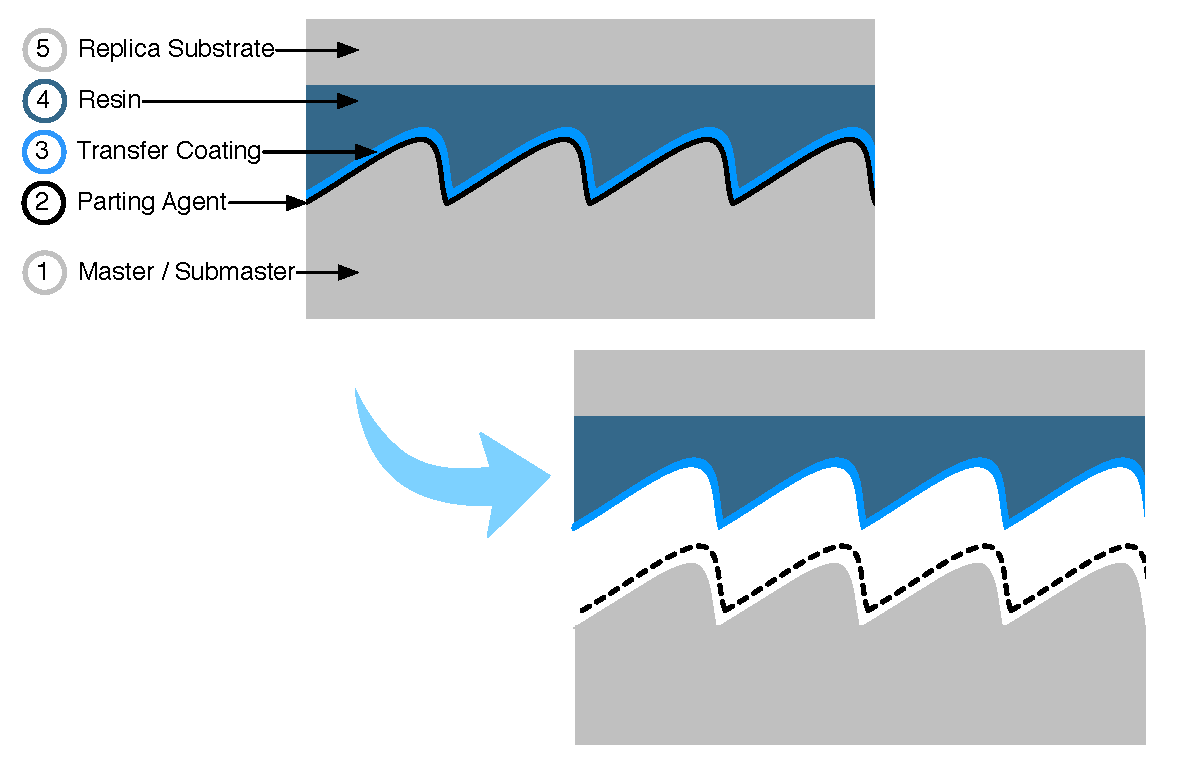
\includegraphics[width=\textwidth]{Chapter3/3c_effectOfProfile/3c_replica.pdf}
   \caption[Master gratings can be replicated using a resin that hardens while in contact with the master (or subsequently, a submaster replicated from the first master).]{Master gratings can be replicated using a resin that hardens while in contact with the master (or subsequently, a submaster replicated from the first master).  First, a parting agent (2) is applied to the surface of the master; it must be thin and uniform otherwise it will affect the profile.  A metallic (aluminum or gold) coating about 1um thick is then applied above the parting agent; this coating will eventually end up as the top surface of the replicated grating, and is called the \emph{transfer coating} (3).  Finally, the replica blank (5) is cemented from above using a resin ($\sim$10um thick) that hardens under UV exposure or over time (4).  Once the resin is cured, the gratings are separated at the parting agent layer, leaving the hardened resin in the shape of the grooves, with the metal coating adhered to the top.  This will produce a mirror image of the master grating; to create a perfect replica, this first replica needs to be replicated again.}
   \label{3c-replication}
\end{figure}

\noindent \textbf{\emph{Holographic Ruling}}

\noindent A more recent technique was invented in the late 1960s for manufacturing gratings faster and with more repeatability.  It uses two sources of coherent light to project a  holographic interference pattern of regular standing waves onto a grating master.  The grating master consists of a photoresist material that is either strengthened or weakened by exposure to light.  After the master has been exposed to the interference pattern for a sufficient time, it is bathed in a developer chemical, which washes away either the exposed or unexposed parts, leaving behind a sinusoidal relief pattern that corresponds to the original intensity of light \cite{Lin82}.

The last groove profile shown in Figure \ref{3c-profile} represents an attempt to turn holographically-ruled sinusoidal gratings into triangular gratings using ion etching to partially eat away the groove surface while holding the finished photoresist master at an angle to the ion beam \cite{Aoy76}.  Another technique for pseudo-blazed holographic gratings is known as Sheridon's Method \cite{She68}, which uses a transparent photoresist exposed to the intersection of a coherent light source with its reflected self (Figure \ref{3c-sheridon}).  Because the master is inclined relative to the interference pattern, the intensity profile is asymmetric and produces a lopsided sinusoidal shape.

\begin{figure}[htbp] %  figure placement: here, top, bottom, or page
   \centering
   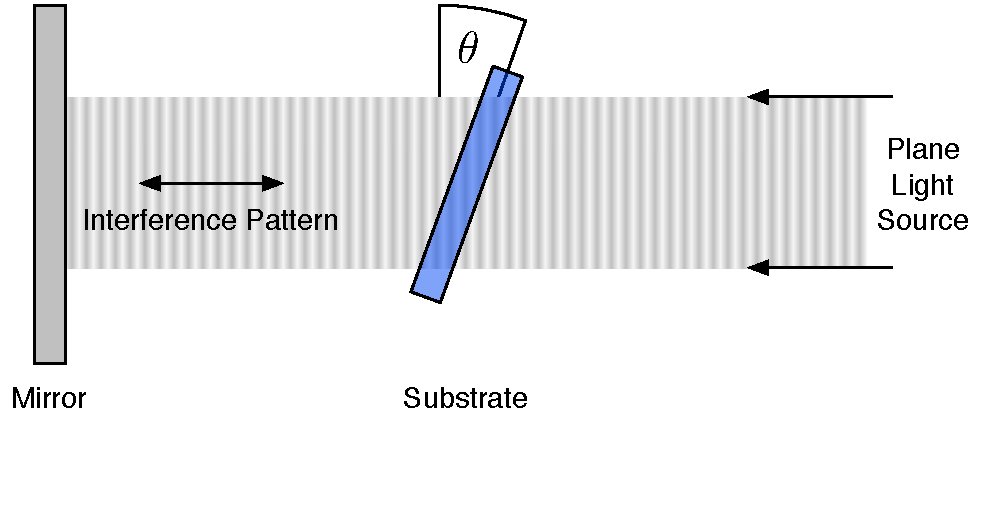
\includegraphics[scale=0.7]{Chapter3/3c_effectOfProfile/3c_sheridon.pdf}
   \caption[The Sheridon technique for recording pseudo-blazed holographic gratings uses a single light beam reflected back on itself to make a regular interference pattern of standing waves.  The master substrate consists of a \emph{transparent} photoresist material that is hardened or weakened by exposure to the light.]{The Sheridon technique for recording pseudo-blazed holographic gratings uses a single light beam reflected back on itself to make a regular interference pattern of standing waves.  The master substrate consists of a \emph{transparent} photoresist material that is hardened or weakened by exposure to the light.  By placing the substrate at an angle $\theta$ to the light path, the light and dark fringes are stretched out parallel to the grating surface; additionally, the angled incidence creates a lopsided sinusoidal intensity pattern that mimics blazed gratings.}
   \label{3c-sheridon}
\end{figure}


\subsection{Profile geometry}
Figure \ref{3c-profile} shows the parameters that describes that describe the geometry of each profile.  In addition to the groove spacing $d$, rectangular gratings are characterized by a groove depth $h$ (or duty cycle) and a groove width $a$.  Ruled triangular gratings are described by their blaze angle $\theta_b$, and the opposite angle (or ``anti-blaze angle'') $\theta_{ab}$.\footnote{Ideally the anti-blaze angle should be 90$\deg$, but it is usually less than 30$\deg$ due to constraints on the ruling tip shape.}  Trapezoidal gratings are described by a groove depth $h$, a groove width $a$, and their blaze and anti-blaze angles $\theta_b$ and $\theta_{ab}$.  Sinusoidal gratings are fully described by just their groove depth $h$, and an assumption of a sinusoidal variation $y(x) = y_0 + \frac{h}{2}\, \sin(2\pi \,x / d)$.

\subsection{Blazed optimization for triangular gratings}
\label{blazeAngle}
The triangular profile in Figure \ref{3c-profile} (b) is much more than an accidental artifact of mechanical ruling.  This shape is optimal for concentrating as much energy as possible into a single order, and therefore boosting the grating efficiency in that order.  Intuitively, we might imagine that to increase efficiency, we should line up the direction of classical ``reflection'' off the majority of the grating surface with the direction of the diffracted ray.  Still thinking classically, we might also want to minimize shadowing in the corners of the grooves. 

The ideal blazed grating meets both of these criteria.  By carefully choosing a blaze angle $\theta_b$ we can -- at least at one wavelength of interest -- line up the specular reflection of the angled surface with the diffraction direction in order $n$.  Using the law of reflection from geometric optics ($\theta_{\mathrm{incident}} = \theta_{\mathrm{reflected}}$), we can easily\footnote{Setting up a ruling engine to correctly and accurately engrave this angle is another story...} derive the optimized condition for a blazed grating.  From the geometry in Figure \ref{3d}, where $N^\prime$ is normal to the angled surface: 
\begin{align}
\theta_{\mathrm{incident}} &= \theta_{\mathrm{reflected}} \\
\theta_2 - \theta_b &= \theta_{2,n} + \theta_b \\
\theta_{2,n} - \theta_{2} &= -2 \theta_b
\end{align}
Applying a trigonometric identity to the grating equation (\ref{gratingEquation}):
\begin{align}
n\lambda / d &= \sin\theta_{2,n} - \sin\theta_{2} \\
\frac{n\lambda}{2d} &= \cos \left( \frac{\theta_{2,n} + \theta_{2}}{2} \right) \sin \left( \frac{\theta_{2,n} - \theta_{2}}{2} \right) \\
\frac{n\lambda}{2d} &= \cos \left( \frac{\theta_{2,n} + \theta_{2}}{2} \right) \sin \left( -\theta_b \right) \\
\end{align}
or
\begin{align}
\label{blazeAngleEqn}
\theta_b = -\arcsin \left(   \frac{n \lambda}{2d \, \cos \left( \frac{\theta_{2,n} + \theta_{2}}{2} \right)}     \right)
\end{align}

\begin{figure}[htbp] %  figure placement: here, top, bottom, or page
   \centering
   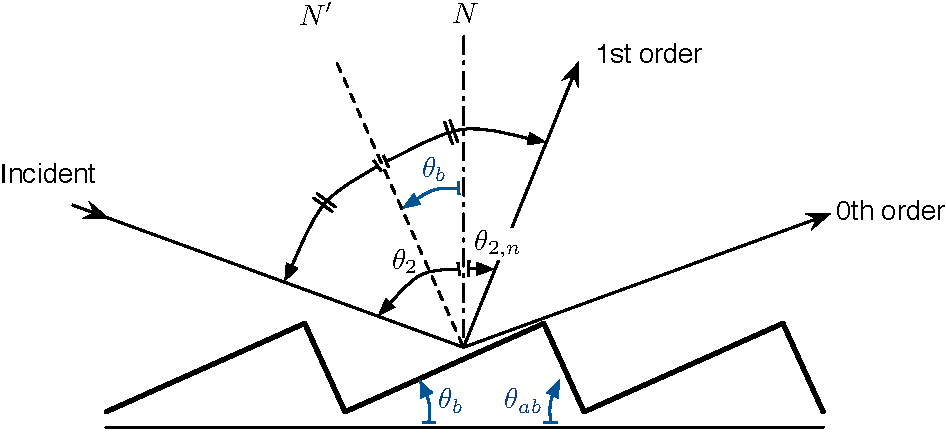
\includegraphics[width=\textwidth]{Chapter3/3d_blazing/3d.pdf} 
   \caption{In the blazed condition, the desired order diffraction angle -- in this case, 1st order -- is aligned with the direction of specular reflection off the groove surfaces.  The angle at the base of the large facet is the \emph{blaze angle} $\theta_b$; the angle at the base of the opposite facet is the \emph{anti-blaze angle} $\theta_{ab}$.}
   \label{3d}
\end{figure}

Textbooks and resources on beamline design universally provide this derivation and formula for the optimal blaze angle $\theta_b$ \cite[page 4-17]{Tho01} \cite[Section 9.1]{Pal05} \cite{Pea97}.  Using efficiency calculations, we confirmed that this intuitive argument is a good approximation for what happens in the full electromagnetic picture; the actual ideal blaze angle is usually slightly but insignificantly lower.  For a 1200 line/mm grating used at an incidence angle of 88 degrees with 400 eV photons in the first inside order ($n=-1$) (Figure \ref{3c-plot}), Equation \eq{blazeAngleEqn} would recommend a blaze angle of 1.67$\deg$.  We used this as the starting point to conduct a software optimization using efficiency calculations, and were only able to increase the 1st order efficiency from 16.2\% to 16.8\% by reducing the blaze angle from 1.67$\deg$ to the optimal 1.46$\deg$.

Because the blaze angle depends on the $n \lambda$ term in the grating equation, a grating optimized for a wavelength $x$ in 1st order will also be optimized for a wavelength $x/2$ in 2nd order (or, in terms of energy, optimization for $x$ eV in 1st order would imply optimization for $2x$ eV in 2nd order).  We can confirm this for the blazed grating in Figure \ref{3c-plot}, where the 1st-order efficiency peak occurs at 450 eV, and the 2nd order efficiency peak occurs near 900 eV.

\begin{figure}[htbp] %  figure placement: here, top, bottom, or page
   \centering
   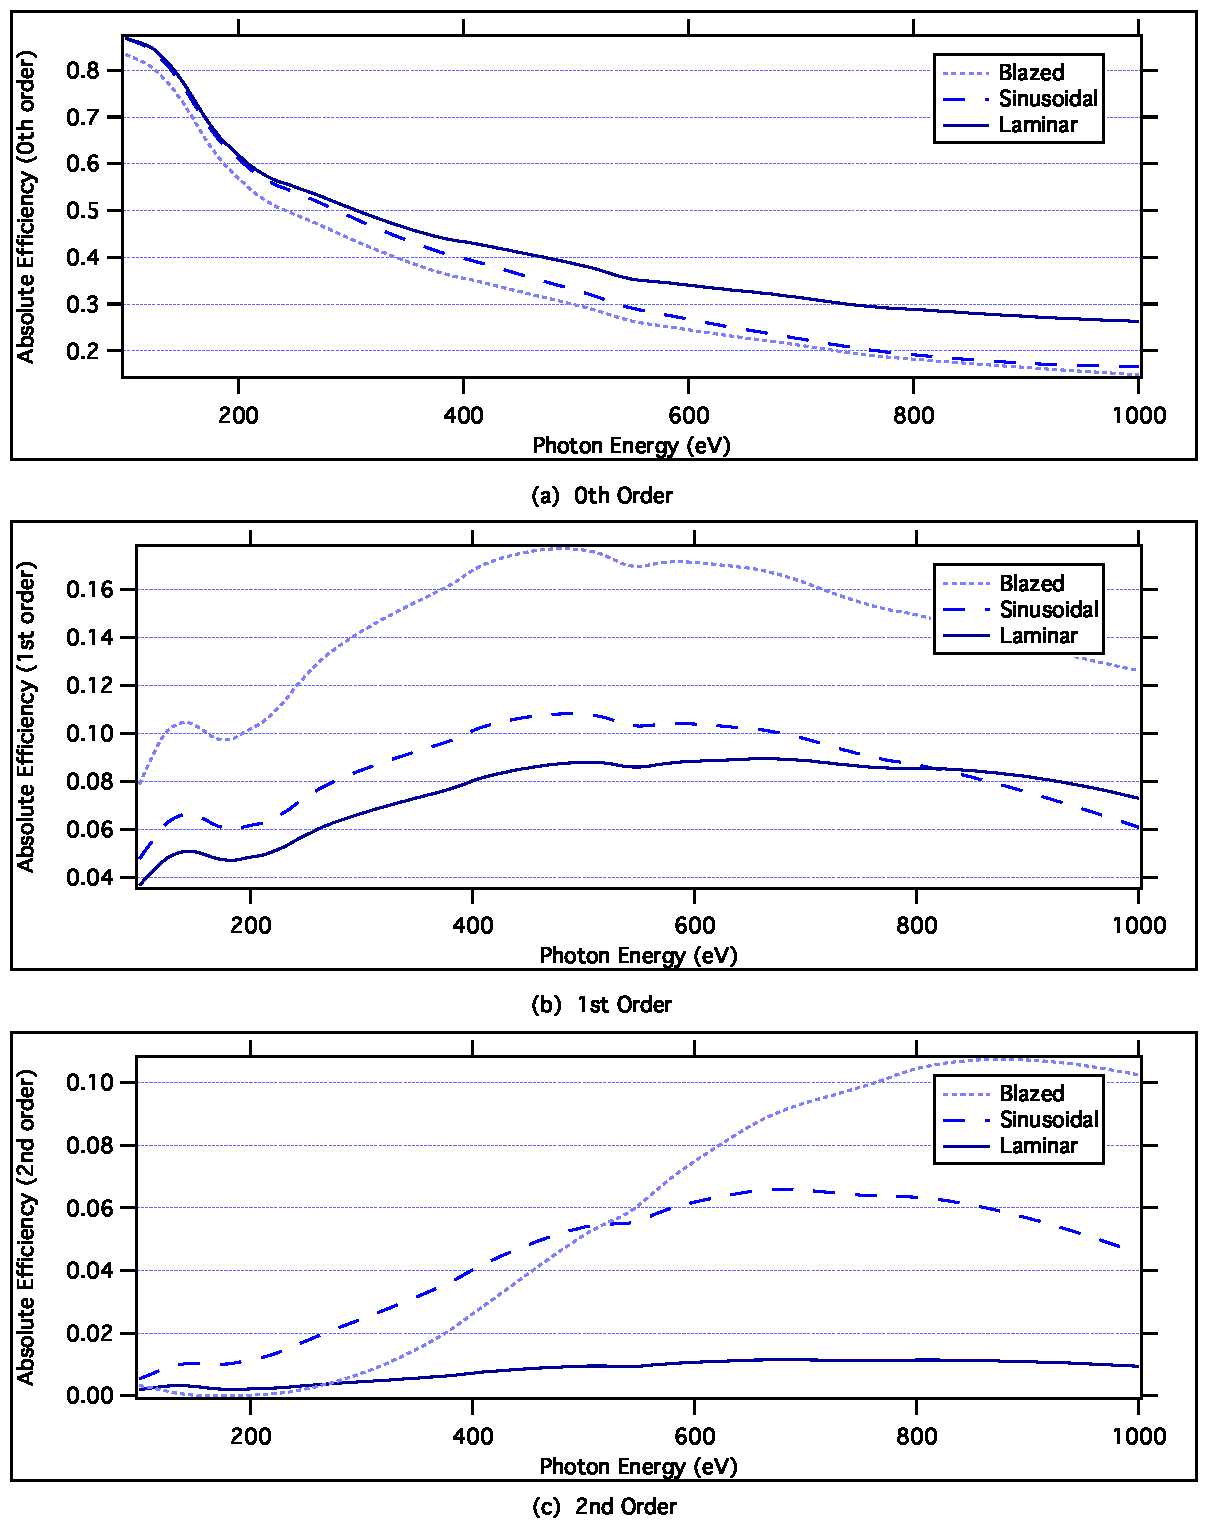
\includegraphics[width=\textwidth]{Chapter3/3c_effectOfProfile/3c_3.pdf} 
   \caption[0th order, 1st order, and 2nd order efficiency of three different groove profiles, all optimized for use at 400 eV.]{0th order, 1st order, and 2nd order efficiency of three different groove profiles, all optimized for use at 400 eV.  The blazed grating is superior in both 1st and 2nd order.  All gratings: 1200 lines/mm, Platinum coating.  Blazed: 1.46$\deg$ angle, 60$\deg$ anti-blaze angle.  Sinusoidal: 13.7 nm groove depth.  Laminar (rectangular): 9.6nm groove depth, 50\% duty cycle. }
   \label{3c-plot}
\end{figure}

\subsection{Efficiency comparison of common profiles}
For comparison, Figure \ref{3c-plot} shows the 0th order, 1st order, and 2nd order efficiency for three common grating profiles: blazed, sinusoidal, and rectangular (commonly referred to as \emph{laminar}).  All three gratings have a groove density of 1200 lines/mm, are shown at an incidence angle of 88 degrees, and have had their geometry optimized for maximum efficiency in 1st-order with 400 eV photons.  (The coating is platinum, and the substrate is quartz [SiO$_2$].)  The blazed grating was optimized by adjusting the blaze angle; the sinusoidal grating by adjusting the groove depth, and the rectangular grating by adjusting the groove depth and assuming a duty cycle of 50\%.

The blazed profile is substantially superior to both the sinusoidal and laminar alternatives.  In first order, even though the efficiency curve peaks near the design energy of 400 eV, the performance is better across the entire range from 100 eV to 1000 eV (and beyond).  The blaze effect causes this curve to be shifted up in energy by a factor of two in 2nd order, so that again the blazed grating out-performs the other profiles, but only above 500 eV.  The sinusoidal grating has relatively flat efficiency across the energy range, even though it still shows the energy-dependence of its optimization for 400 eV.   (We have chosen a platinum coating for these examples since its reflectivity is relatively constant across the energy range (Figure \ref{3g-2}).  The small universal dip in efficiency at 180 eV is due to a drop in the Pt reflectivity here.)

\section{Effect of groove density}
Because the groove density directly affects the angular dispersion, using a higher-density grating is the most direct path to designing a higher-resolution instrument (Section \ref{resolutionGoals}).  Unfortunately, Figure \ref{3e} shows that increasing the groove density universally decreases the grating efficiency in all orders except the 0th order, even when the remaining parameters are adjusted to keep the grating optimized.  This turns out to be true, not only in this example for two grating profiles, but as a general principle.  Intuitively, we can argue that as the groove density approaches infinite, the grating will look more and more like a flat mirror -- with microstructure becoming smaller and smaller.  Therefore, it makes sense that the amount of light in the 0th-order specular reflection will increase at the expense of the diffracted orders.

Figure \ref{3e-2} explores the groove density effect in more detail, with an efficiency spectrum for a series of blazed gratings from 300 lines/mm to 2700 lines/mm, all optimized for 400 eV at 88$\deg$ incidence.  It confirms that as the groove density increases, the 0th order efficiency increases, and the $n\neq0$ order efficiencies decrease.  However, one fortunate outcome is that as the groove density increases, the width of the efficiency peak caused by the blazing optimization becomes wider; therefore, higher groove-density blazed gratings can be used optimally over a wider energy range than low-density gratings.
	
\begin{figure}[htbp] %  figure placement: here, top, bottom, or page
   \centering
   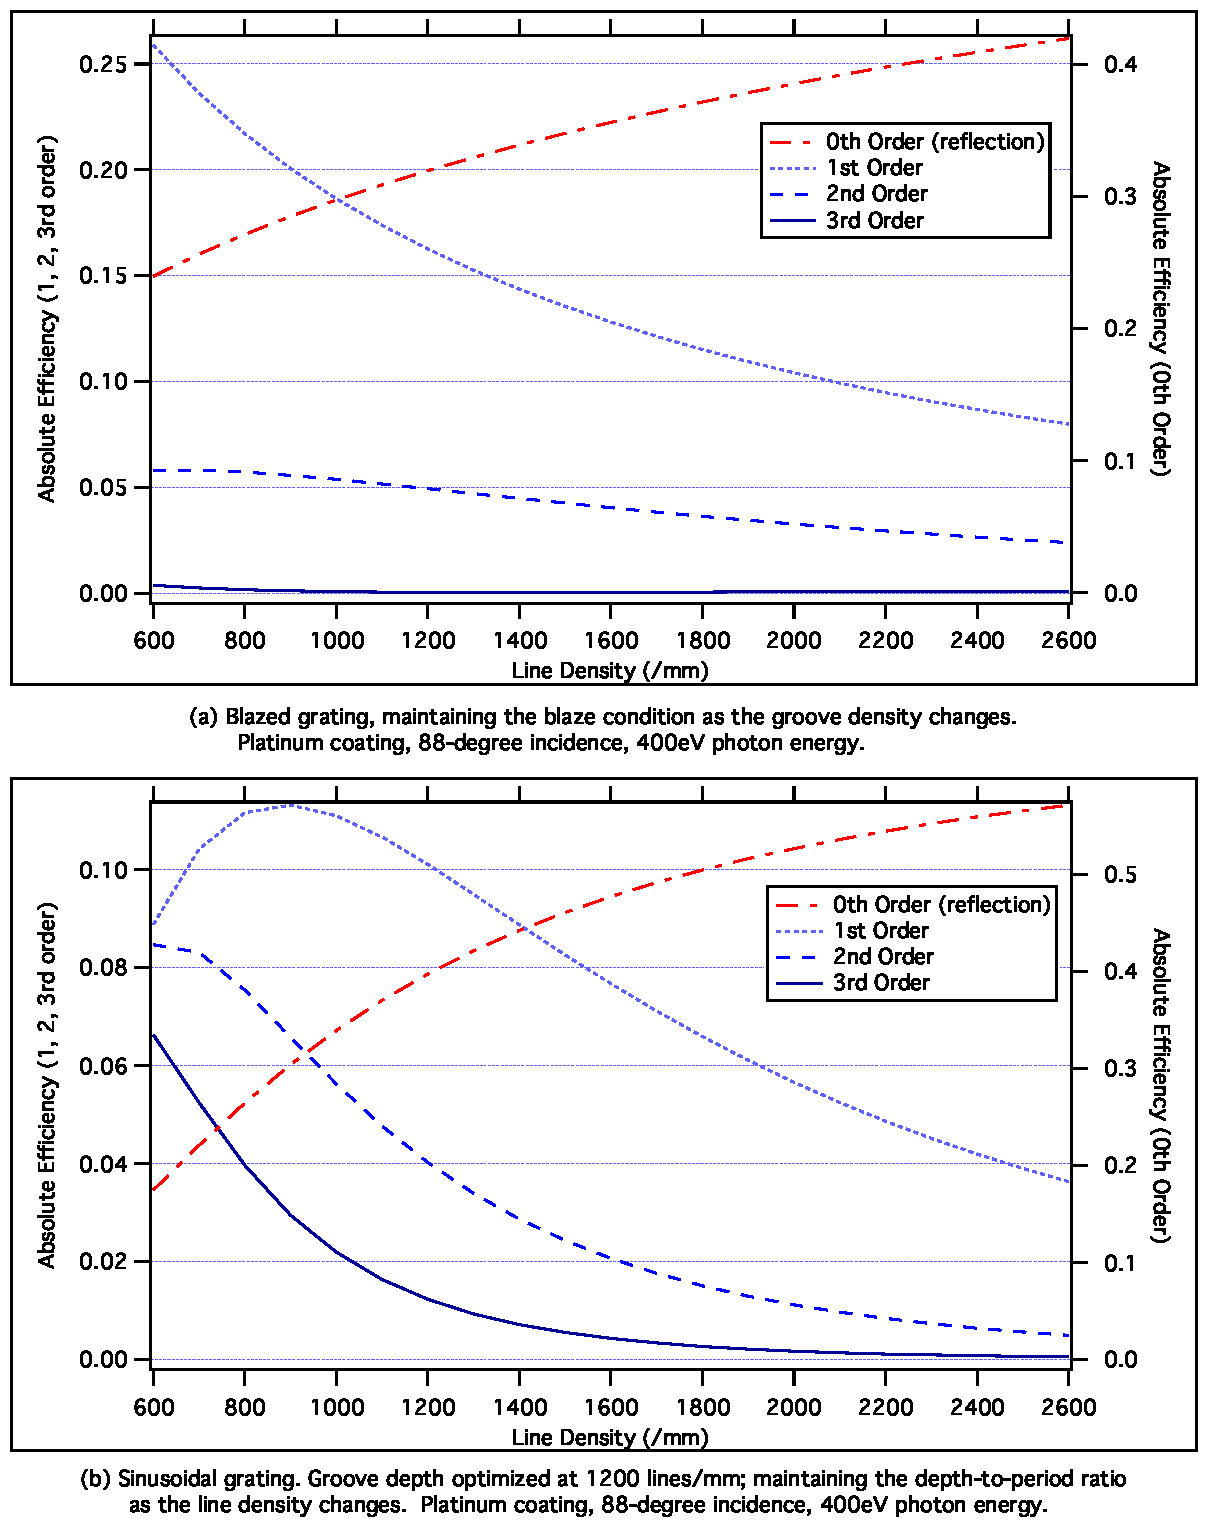
\includegraphics[width=\textwidth]{Chapter3/3e_effectOfGrooveDensity/3e.pdf} 
   \caption[Increasing the groove density always decreases the diffraction efficiency -- at least for all the useful orders ($n \neq 0$).]{Increasing the groove density always decreases the diffraction efficiency -- at least for all the useful orders ($n \neq 0$).  In these plots, we tried to control for inter-related factors: For the blazed grating in (a), the blaze angle has been adjusted with the groove density (using Equation \protect \eq{blazeAngleEqn}) to maintain the on-blaze condition.  In (b), the sinusoidal grating depth was optimized at 1200 lines/mm, and then the depth-to-period ratio was maintained across changes to the groove density.}
   \label{3e}
\end{figure}

\begin{figure}[htbp] %  figure placement: here, top, bottom, or page
   \centering
   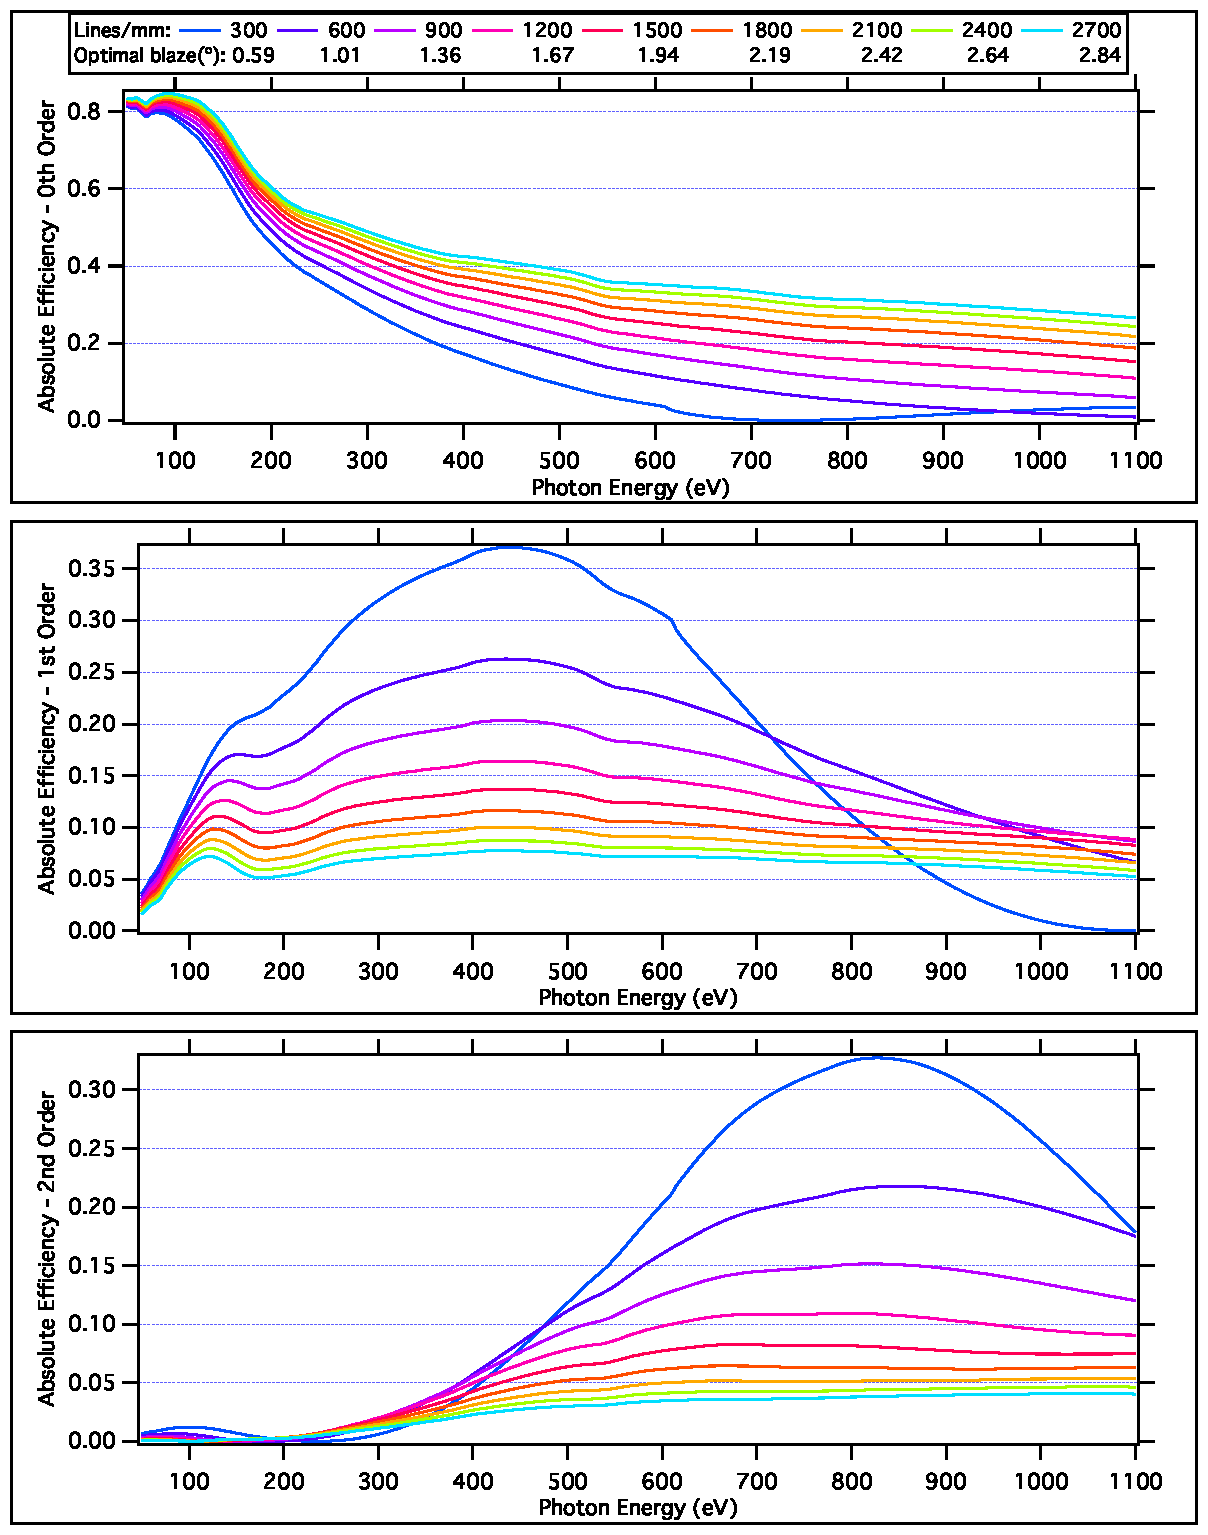
\includegraphics[width=\textwidth]{Chapter3/3e_effectOfGrooveDensity/3e-2.pdf} 
   \caption[0th order, 1st order, and 2nd order efficiency as a function of energy, for a range of groove densities from 300 to 2700 lines/mm. As the groove density increases, the maximum achievable efficiency drops, but the bandwidth of the blaze-optimization peak becomes wider.]{0th order, 1st order, and 2nd order efficiency as a function of energy, for a range of groove densities from 300 to 2700 lines/mm.  All gratings are triangular, platinum-coated, with an optimal blaze angle dependent on the groove density according to Equation \protect \eq{blazeAngleEqn}.  (Blaze angles are shown in the legend.)  As the groove density increases, the maximum achievable efficiency drops, but the bandwidth of the blaze-optimization peak becomes wider.}
   \label{3e-2}
\end{figure}

\section{Effect of coating thickness}
Gratings intended for use in soft x-ray instruments are manufactured on precision-ground  blanks, usually consisting of fused quartz (SiO$_2$) or other amorphous glasses.  The insulating (dielectric) blank is coated in a layer of metal, where the smoothness of the surface is absolutely critical.  Often gold is used as a first coating, since it can be applied with very low roughness, and because it provides a soft layer in which to rule the grooves.  If another type of coating is required (such as nickel and platinum, in our case), these coatings are applied on top of the gold after ruling.

The required thickness of the coating is another question that can be answered by efficiency calculations.   Thin coatings can be applied more smoothly than thick ones \cite{Pea97}, so the question is: how thick must a coating be for a given photon energy and incidence angle, so that photons are fully reflected or absorbed before reaching the substrate interface?  If the coating is too thin, the absorption characteristics of the glass oxide substrate will start to show up in the efficiency spectrum.

\begin{figure}[htbp] %  figure placement: here, top, bottom, or page
   \centering
   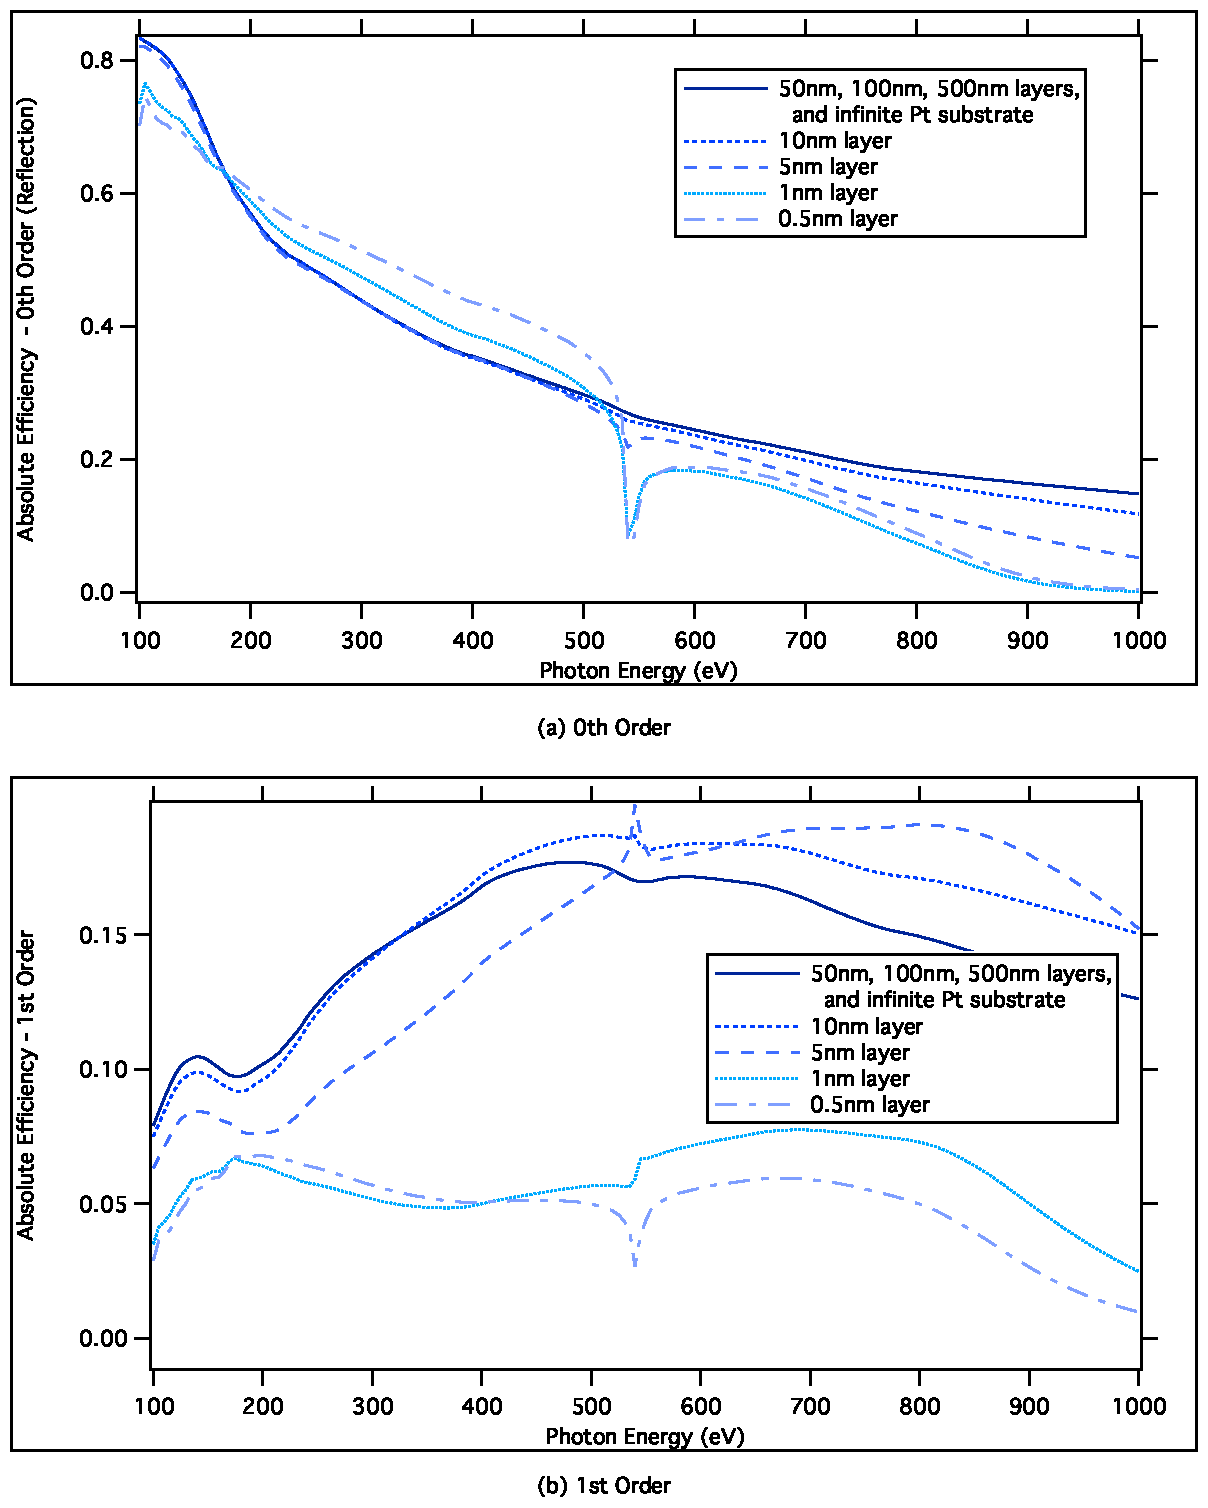
\includegraphics[width=\textwidth]{Chapter3/3f_coatingThickness/3f.pdf} 
   \caption[In the soft x-ray regime under grazing incidence, metal-coated dielectric gratings are indistinguishable from pure metal gratings\ldots as long as the coating is thicker than $\sim$ 20 nm.]{In the soft x-ray regime under grazing incidence, metal-coated dielectric gratings are indistinguishable from pure metal gratings\ldots as long as the coating is thicker than $\sim$ 20 nm.  (The exact required thickness depends on the material, photon energy, and incidence angle).  These calculations show Pt coatings of varying thickness over an SiO$_2$ substrate, as well as an infinitely thick pure Pt grating.  (Blazed grating, 1200 lines/mm, 1.46$\deg$ blaze angle, 88$\deg$ incidence.}
   \label{3f}
\end{figure}

Figure \ref{3f} shows calculations for various thicknesses of platinum coatings above an SiO$_2$ substrate, compared with a theoretical solid platinum grating of infinite thickness.  The 0.5nm and 1nm coatings show the oxygen absorption edge at 525 eV, as well as significantly reduced reflectivity over the whole energy range.  The 5 nm layer shows a thin-film interference effect that actually boosts the efficiency above 600 eV.\footnote{The sharp peak in this spectrum at 525 eV might be anomalous; the Henke data used to derive the complex refractive index of all these materials is not accurate in the vicinity of absorption edges.}  As we should expect, at a thickness of 50nm and above, the coated gratings become indistinguishable from an infinitely-thick platinum substrate.  

In general, the required minimum thickness will depend on the photon energy, incidence angle, and the x-ray form factor of the coating material -- all of which affect the x-ray penetration depth.  These results show that for thin coatings, the efficiency calculations are able to rigorously incorporate the effects of interference and absorption at the interface with the substrate.

\section{Comparison of coating materials}
All materials suffer from inherently low reflectivity at soft x-ray energies.  Even when gratings are used at grazing incidence, designers must carefully choose coating materials to maximize efficiency considering the desired wavelength range of the instrument.  (This becomes particularly frustrating when a material with otherwise high reflectivity has an absorption edge right in the middle of the region of interest.)

To help in selecting materials, Figures \ref{3g} and \ref{3g-2} show several possibly grating coatings: carbon, nickel, gold, platinum, and iridium.  (Figure \ref{3g} shows the reflectivity of a plain mirror made out of these materials over the energy range from 100 to  1000 eV, at 88$\deg$ grazing incidence.  Figure \ref{3g-2} compares the mirror reflectivity with the 0th order and 1st order efficiency of a sinusoidal grating, which had its groove depth optimized for 400 eV.)

\begin{figure}[htbp] %  figure placement: here, top, bottom, or page
   \centering
   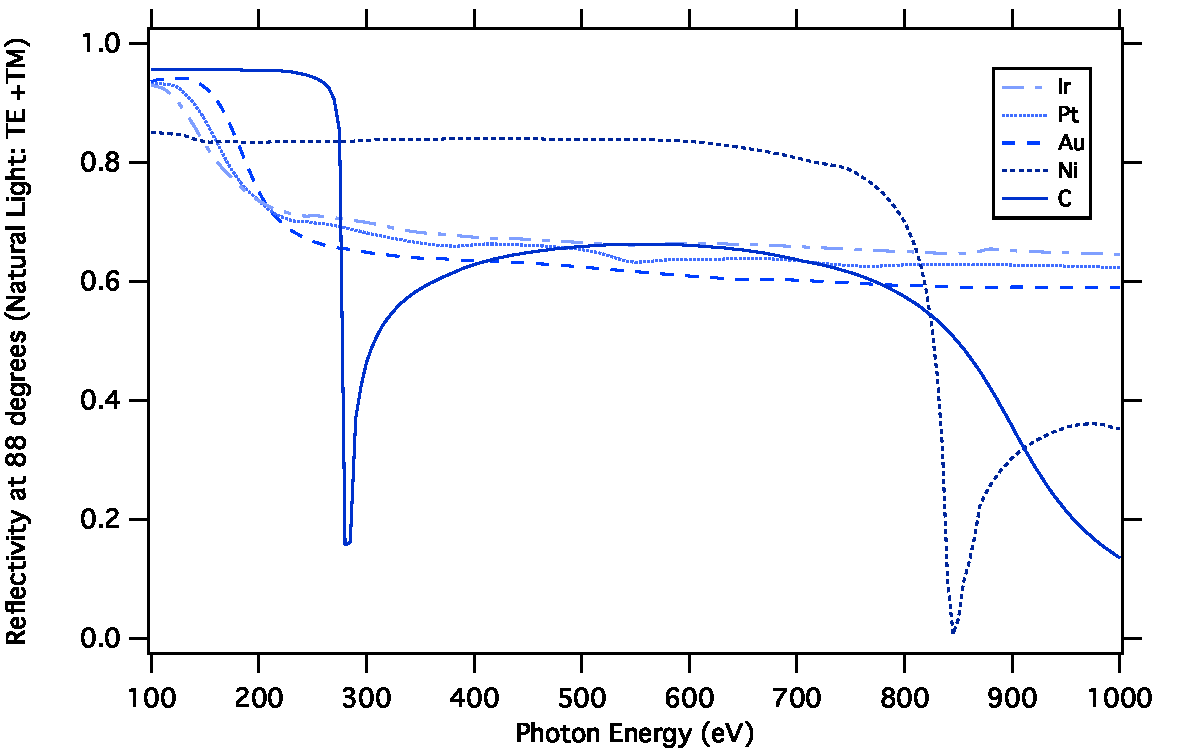
\includegraphics[width=\textwidth]{Chapter3/3g_coatingMaterial/3g_reflectivity.pdf} 
   \caption[The reflectivity of a pure mirror at grazing incidence (88$\deg$), as a function of photon energy.]{The reflectivity of a pure mirror at grazing incidence (88$\deg$), as a function of photon energy.  Lighter elements like carbon and nickel have the highest peak reflectivity, but have strong absorption features.  Heavier metals, particularly those within the platinum group, have reasonable reflectivity over the entire soft x-ray region of interest.  Up to 200 eV, gold has a higher reflectivity than Pt and Ir. }
   \label{3g}
\end{figure}

\begin{figure}[htbp] %  figure placement: here, top, bottom, or page
   \centering
   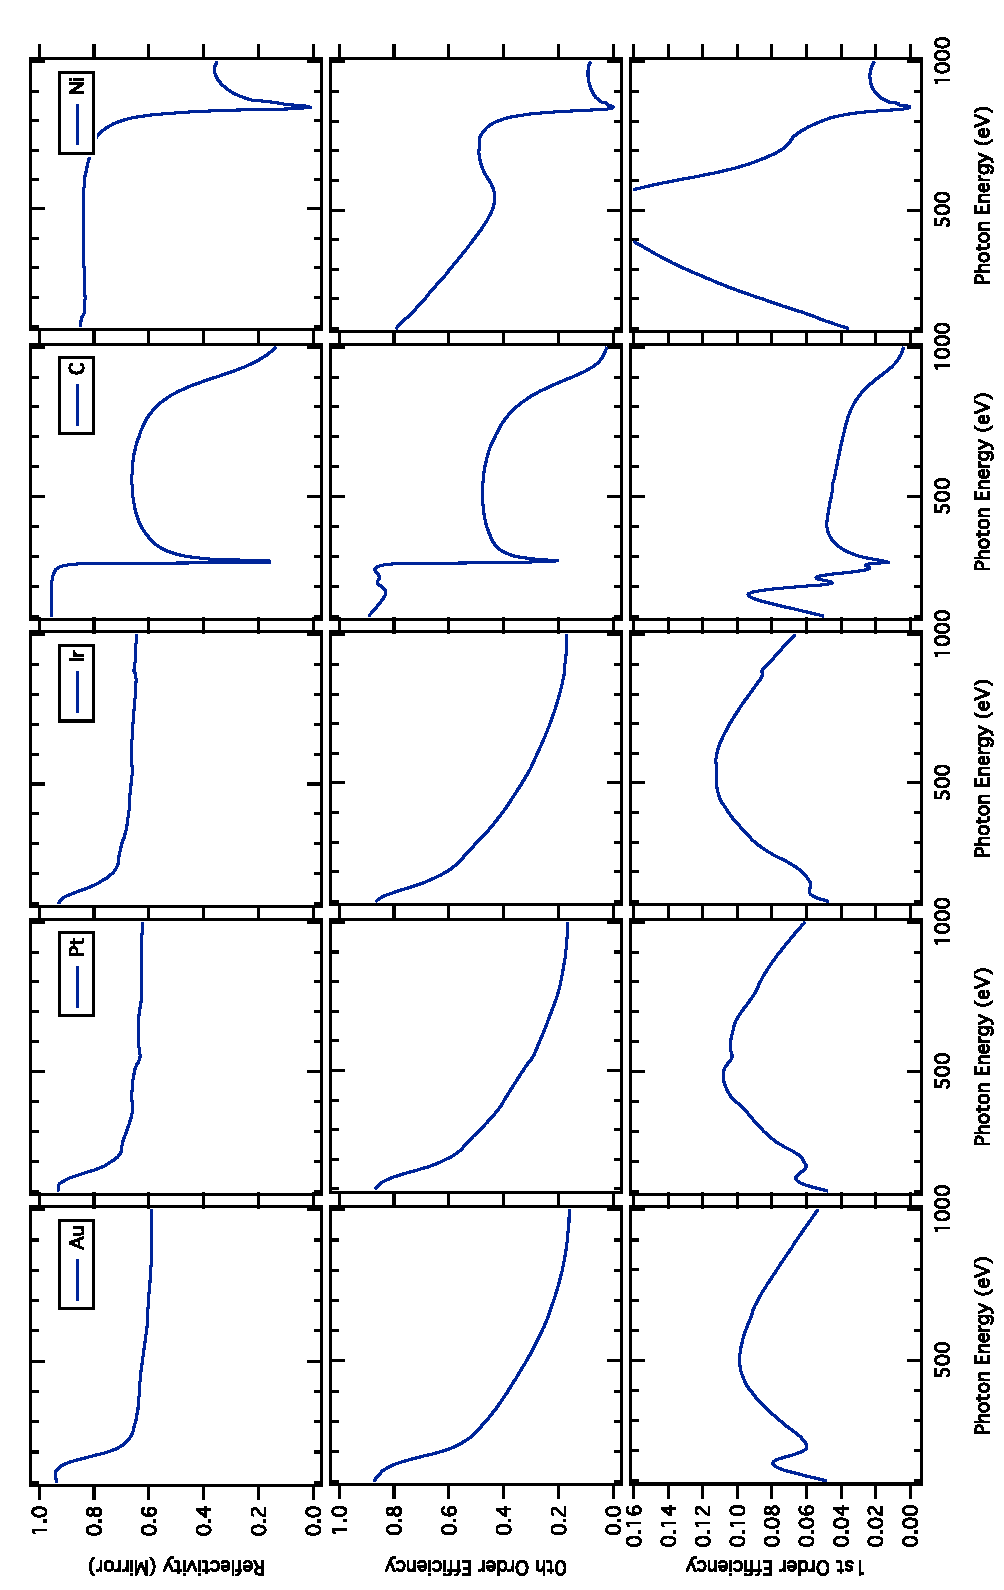
\includegraphics[scale=0.77]{Chapter3/3g_coatingMaterial/3g_multiview.pdf} 
   \caption[A comparison of the mirror reflectivity, 0th order, and 1st order efficiency for different coating materials, as a function of photon energy.]{A comparison of the mirror reflectivity, 0th order, and 1st order efficiency for different coating materials, as a function of photon energy.  (Gratings: Sinusoidal profile, 88$\deg$ incidence angle, 1200 lines/mm, 13.7 nm groove depth.)  Note that the 1st order efficiency has energy-dependent features that are not visible in the simple reflectivity.}
   \label{3g-2}
\end{figure}

The heavy precious metals (Au, Pt, Ir) are commonly chosen for grating coatings because they have a relatively constant reflectivity over this energy range.  This is because their core-level electrons are so tightly bound that their strongest absorption features occur well above the soft x-ray range.  (For example, the Pt K~1s absorption edge is at 78.4 keV.)  Their outer-shell electrons fall within the soft x-ray range (for example, the platinum N and O transitions), but these absorption features are not nearly as strong, and therefore do not seriously affect the reflectivity.  Gold has better reflectivity than Pt and Ir below 200 eV, and also has the previously-mentioned desirable property of being easy to apply smoothly and rule mechanically.  Above 200 eV, platinum has been the de-facto choice for high-energy wide-bandwidth gratings for many years.  Iridium (and rhodium, not shown) actually have even better reflectivity and corrosion resistance than platinum, and are becoming standard coating options with some manufacturers.

In contrast, carbon and nickel offer much higher reflectivity over some parts of this energy range, but unfortunately have strong absorption features right in the middle.  The carbon K 1s absorption edge at 284 eV makes it restricted to, but excellent for, low-energy applications.  The nickel L$_2$/L$_3$ edges do not occur until 870/853 eV, and Figure \ref{3g-2} seems to suggest that nickel would be the clear winner over much of the soft x-ray range.  This prompted us to use it for two of the REIXS spectrometer gratings, with one obvious but unforeseen consequence (Section \ref{nickelOxidation}).

Not shown in these plots, silicon also has a very high reflectivity up to its L$_2$/L$_3$ absorption edge at 100 eV. Therefore, bare Si and SiO$_2$ mirrors are often used for extreme ultra-violet (EUV) and very low-energy soft x-ray beamlines \cite{Pea97}; Si-coated gratings might be useful here as well.

\section{Effect of photon energy / wavelength}
The energy-dependence (or wavelength-dependence) of grating efficiency is shown in many of the previous plots, where we display the efficiency as a function of photon energy.  However, it is impossible to isolate trends for this relationship on its own, because the photon energy is inherently coupled to the grating efficiency in multiple ways.  For starters, the complex refractive indexes of grating materials always vary as a function of energy.  Additionally, the photon energy also determines the angle of the outgoing diffraction orders, which can be seen in both the Rayleigh expansion for the total field, and in the simplified grating equation \eq{gratingEquation}.  Therefore, optimizations for geometry parameters that depend on outgoing angles -- like the blaze angle and groove depth -- are inherently coupled to the photon energy.  The plots in Figure \ref{3g-2} highlight this by showing the difference between the energy-dependent reflectivity of a plain flat mirror, versus the more complicated diffraction efficiency.

\section{Effect of incidence angle}
\label{incidenceAngle}
\label{TER}
In the soft x-ray regime, the real part of the refractive index for metals is less than unity.  This means that the phase velocity for light in the material is actually \emph{faster} than the speed of light in a vacuum.\footnote{Because the refractive index changes with wavelength, dispersion causes a \emph{group velocity} $v_g < c$, therefore Einstein's speed limit is not violated.}  As mentioned in Section \ref{TER-intro}, we can exploit this phenomenon to increase the reflectivity of gratings and mirrors by using them at grazing incidence, creating what is sometimes referred to non-rigourously as \emph{``total external reflection''} (TER).

Total internal reflection (TIR) happens in conventional materials when a light ray travels from a slower optical medium (refractive index $n_2$) toward a faster optical medium (refractive index $n_1 < n_2$).  Snell's law of refraction would relate the angles of the incident ($\theta_2$) and transmitted ($\theta_1$) waves:
\begin{align}
n_2 \sin \theta_2 &= n_1 \sin \theta_1 \\
\sin \theta_1 &= \frac{n_2}{n_1} \sin \theta_2
\end{align}
By choosing an incident angle $\theta_2$ for which there is no possible solution to $\theta_1$, we can ensure that there is no transmitted wave -- the incident wave must be completely reflected.
\begin{align}
 \frac{n_2}{n_1} \sin \theta_2 &> 1
\end{align}
This will happen for all incident angles $\theta_2$ beyond a critical angle:
\begin{align}
\theta_{\mathrm{critical}} &= \arcsin \left( \frac{n_1}{n_2} \right)
\end{align}

In the case of soft x-ray mirrors and gratings, if we make a crude approximation and ignore the imaginary component of the mirror's refractive index, the same situation happens when light from the (slower) vacuum is incident on the (faster) medium of the mirror.\footnote{This assumption is necessary because Snell's law in the form $n_1 \sin \theta_1 = n_2 \sin \theta_2$ only makes sense for real $n$.  If $n_1$ and $\theta_1$ were real, but the mirror's $n_2$ was complex, this would require a complex ``angle'' $\theta_2$, which would have no direct physical interpretation.}
% TODO: really no physical interpretation?
Here the vacuum refractive index is $\nu_2=n_2=1$, and the mirror refractive index is $\nu_1\approx n_1<1$.  (For example, at 410 eV, the real part of the refractive index of platinum is $n_1 = 0.99321$.)  We can therefore calculate the critical angle for \emph{total external reflection}; for incident angles larger than this, there should be no transmitted wave into the mirror:
\begin{align}
\theta_{\mathrm{critical}} &= \arcsin \left( n_1 \right)
\end{align}
(where $n_1$ is the real part of the mirror's complex refractive index.)  Critical angles for the coatings in Figure \ref{3g-2} at 410 eV are given in Table \ref{3i-2}.

\begin{table}[p]
   \centering
   \topcaption{Critical incidence angles for ``total external reflection'' at 410 eV for the mirror and grating coatings shown in Figure \ref{3g-2}.}
   \begin{tabular}{@{} r c @{}} % Column formatting, @{} suppresses leading/trailing space
\toprule
Material    & $\theta_{\mathrm{critical}}$ for TER ($\deg$)\\
\midrule
Carbon (C) & 85.92\\
Nickel (Ni) & 83.20\\
Gold (Au)& 83.85\\
Platinum (Pt)& 83.32\\
Iridium (Ir)& 83.10\\
\bottomrule
   \end{tabular}
   \label{3i-2}
\end{table}

\begin{figure}[p] %  figure placement: here, top, bottom, or page
   \centering
   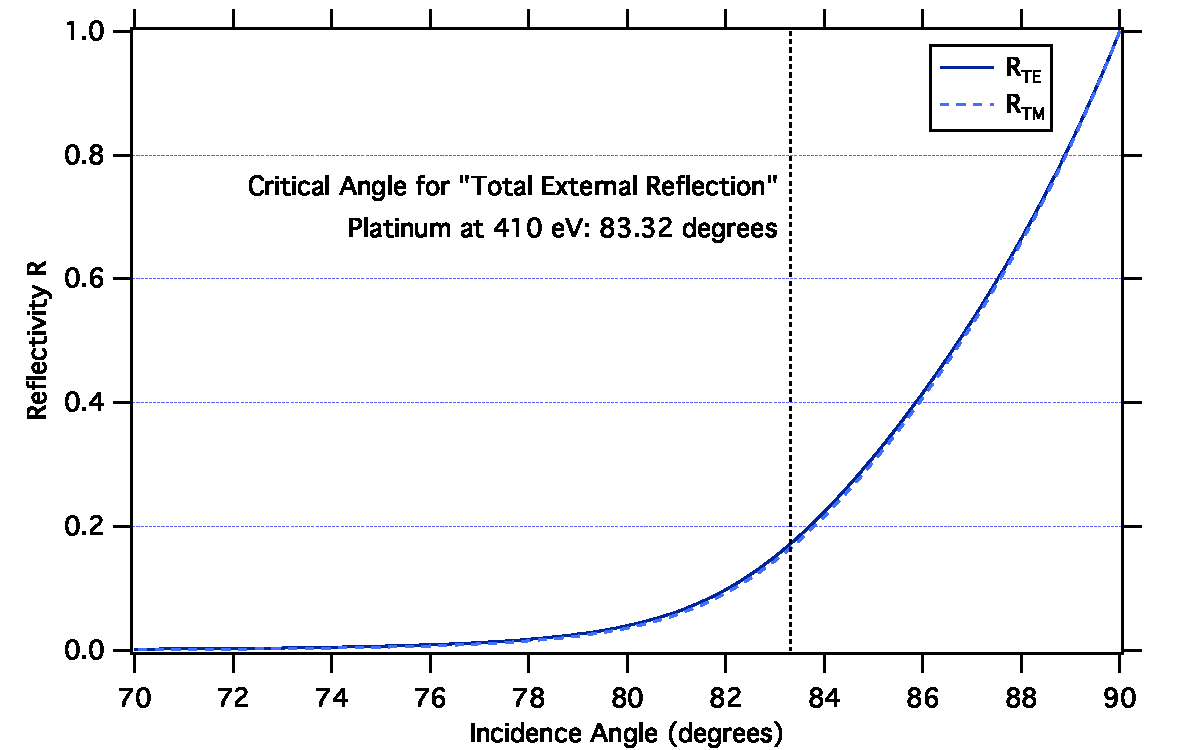
\includegraphics[width=\textwidth]{Chapter3/3i_incidenceAngle/reflectivityVsAngle.pdf} 
   \caption[The reflectivity of a perfect platinum mirror as a function of incidence angle at 410 eV, calculated using the complex refractive index and the complex Fresnel equations.]{The reflectivity of a perfect platinum mirror as a function of incidence angle at 410 eV, calculated using the complex refractive index and the complex Fresnel equations.  The ``total external reflection'' approximation suggests a critical angle of 83.3$\deg$ for total reflection, but due to absorption within the material, the reflectivity only reaches 1 at complete grazing incidence (90$\deg$).  There is no substantial difference between TE and TM polarization.}
   \label{reflectionVsAngle}
\end{figure}

Because we ignored the imaginary component $i \beta$ of the full refractive index ($\nu = n + i \beta$), the concept of TER is just an approximation for what happens in the rigorous electromagnetic picture.  The imaginary component represents absorption of the electromagnetic wave within the material, and as a result, no soft x-ray mirrors are ever totally reflecting -- Figure \ref{reflectionVsAngle} shows that a reflectivity of 1 only occurs at complete grazing incidence (90$\deg$).  Reference \cite{Fow89} gives a rigorous derivation of reflection and transmission from absorbing materials: the reflection coefficients for TE and TM polarization, from a material with complex refractive index $\nu$ at incidence angle $\theta$, are known as the \emph{complex Fresnel equations}:
\begin{align}
\cos \phi &\equiv \sqrt{1 - \frac{\sin^2 \theta}{\nu^2} } \\
\label{eqnFresnelTE}
r_{TE} &=     \frac{\cos \theta - \nu \cos \phi}     {\cos \theta + \nu \cos \phi} \\
\label{eqnFresnelTM}
r_{TM} &=    \frac{-\nu \cos \theta + \cos \phi}              {\nu \cos \theta + \cos \phi}
\end{align}
In general, the reflection coefficients $r_{TE}$ and $r_{TM}$ are also complex, so they give both the amplitude and phase shift of the reflected electric field vector.  The reflectivity $R$ is given by the squared magnitude of the reflection coefficient:
\begin{align}
R_{TE} &= | r_{TE} | ^2 =  r_{TE} \, r_{TE}^\ast \\
R_{TM} &= | r_{TM} | ^2 = r_{TM} \, r_{TM}^\ast
\end{align}
These are plotted in Figure \ref{reflectionVsAngle} as a function of incidence angle for a smooth platinum mirror at 410 eV.

Moving from mirrors to gratings, Figure \ref{3i} shows the effect of incidence angle on diffraction efficiency for several different geometry profiles.  Even though TER is a crude approximation, this figure does confirm that the grating efficiencies in the 0th, 1st, and 2nd orders are indeed extremely low below platinum's ``critical incidence angle'' of 83.3$\deg$.    By comparison with the mirror plot in Figure \ref{reflectionVsAngle}, we might expect that as the incidence angle becomes more and more grazing, the efficiency should increase continuously\ldots and that is certainly the case for the $n=0$ order.  However, this turns out to be not true for the remaining orders; \emph{there is actually an optimal incidence angle below $90\deg$ where efficiency is maximized}.  At first glance, it might seem like this is an accidental side-effect of the blazed optimization; since the optimal blaze angle depends on the incidence angle, it might have been possible that all the gratings in Figure \ref{3i} had their geometry optimized for a sub-$90\deg$ incidence angle.  However, by exploring the effect of incidence angle on efficiency over a range of blaze angles, Figure \ref{3i-2} dispels this idea; it shows that for $n\neq 0$ orders, there is indeed an optimal incidence angle, which depends only on the groove density (period) and the energy.

\begin{figure}[htbp] %  figure placement: here, top, bottom, or page
   \centering
   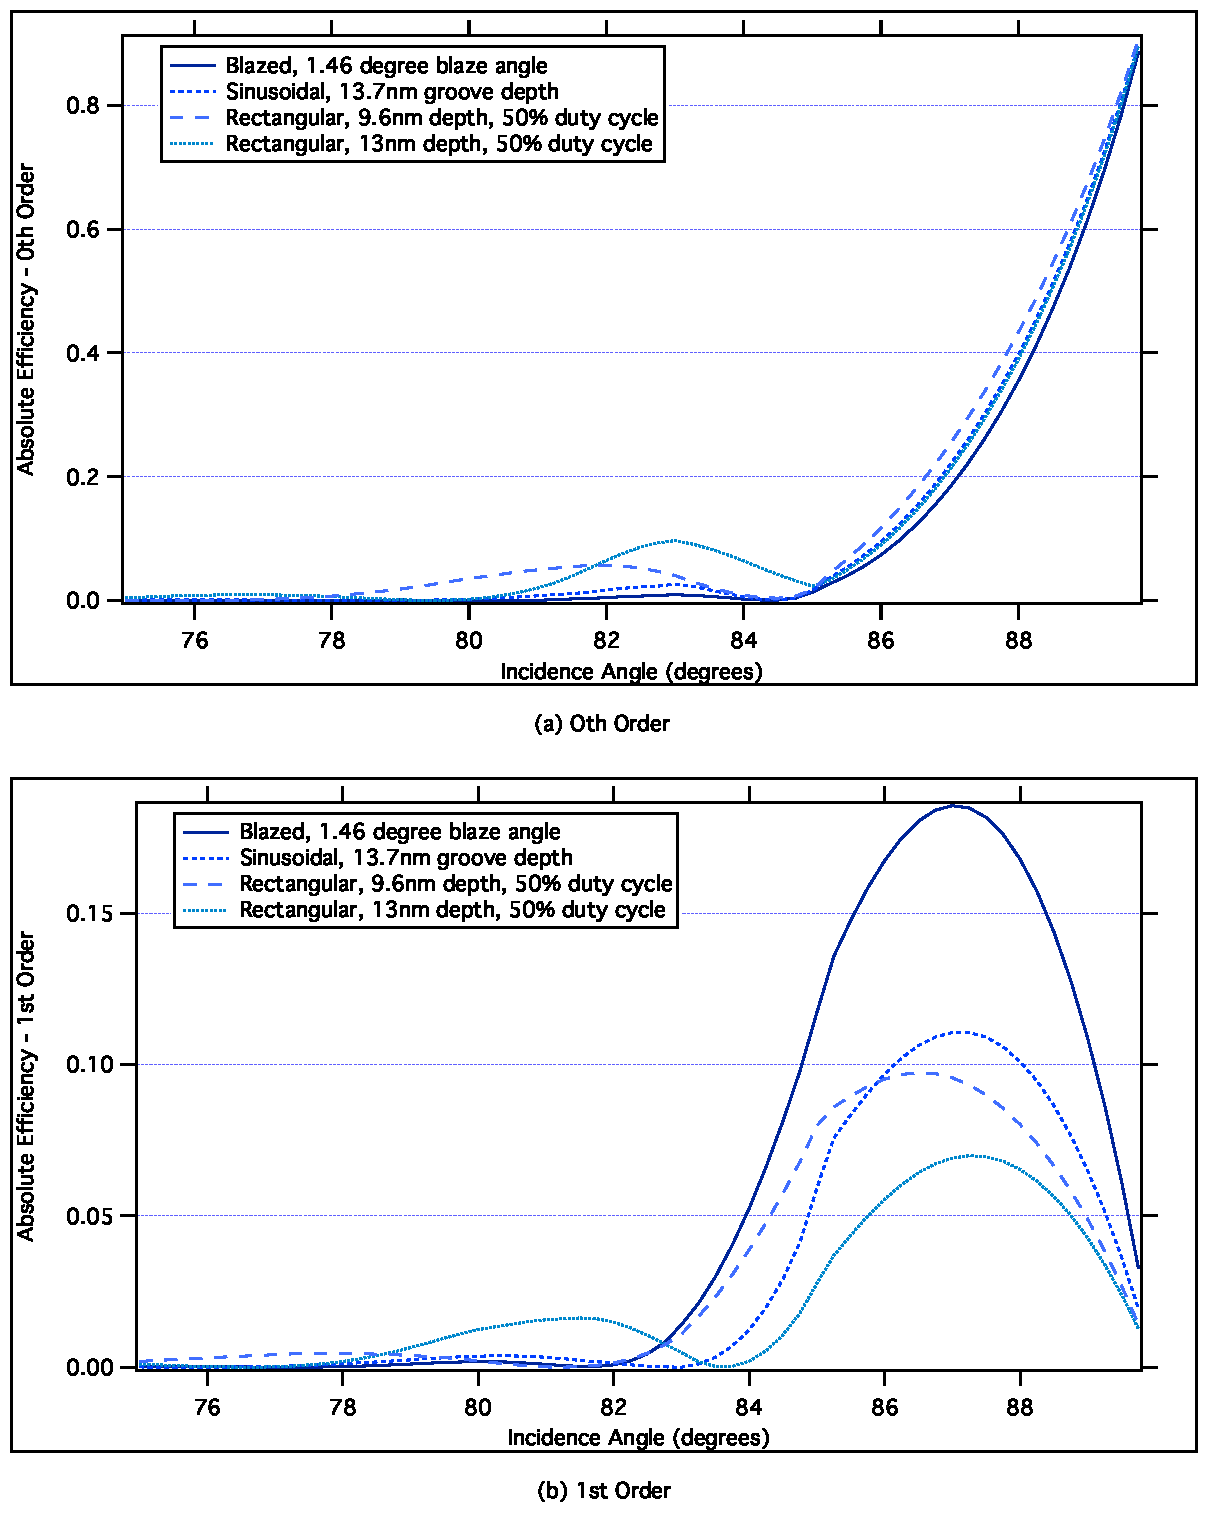
\includegraphics[width=\textwidth]{Chapter3/3i_incidenceAngle/3i_variousGratings.pdf} 
   \caption[The effect of incidence angle on diffraction efficiency for various grating profiles.  While the 0th order efficiency/reflectivity always increases as the incident light becomes more grazing, there is an optimal incidence angle below 90$\deg$ for higher-order light.]{The effect of incidence angle on diffraction efficiency for various grating profiles.  While the 0th order efficiency/reflectivity always increases as the incident light becomes more grazing, there is an optimal incidence angle below 90$\deg$ for higher-order light.  The critical angle for total external reflection in Platinum is 83.3$\deg$; clearly both the 0th-order and 1st-order efficiency drop off significantly below this angle. (Gratings: 1200 lines/mm, platinum coating, 400 eV; blaze angles and profiles as indicated.)}
   \label{3i}
\end{figure}

\begin{figure}[htbp] %  figure placement: here, top, bottom, or page
   \centering
   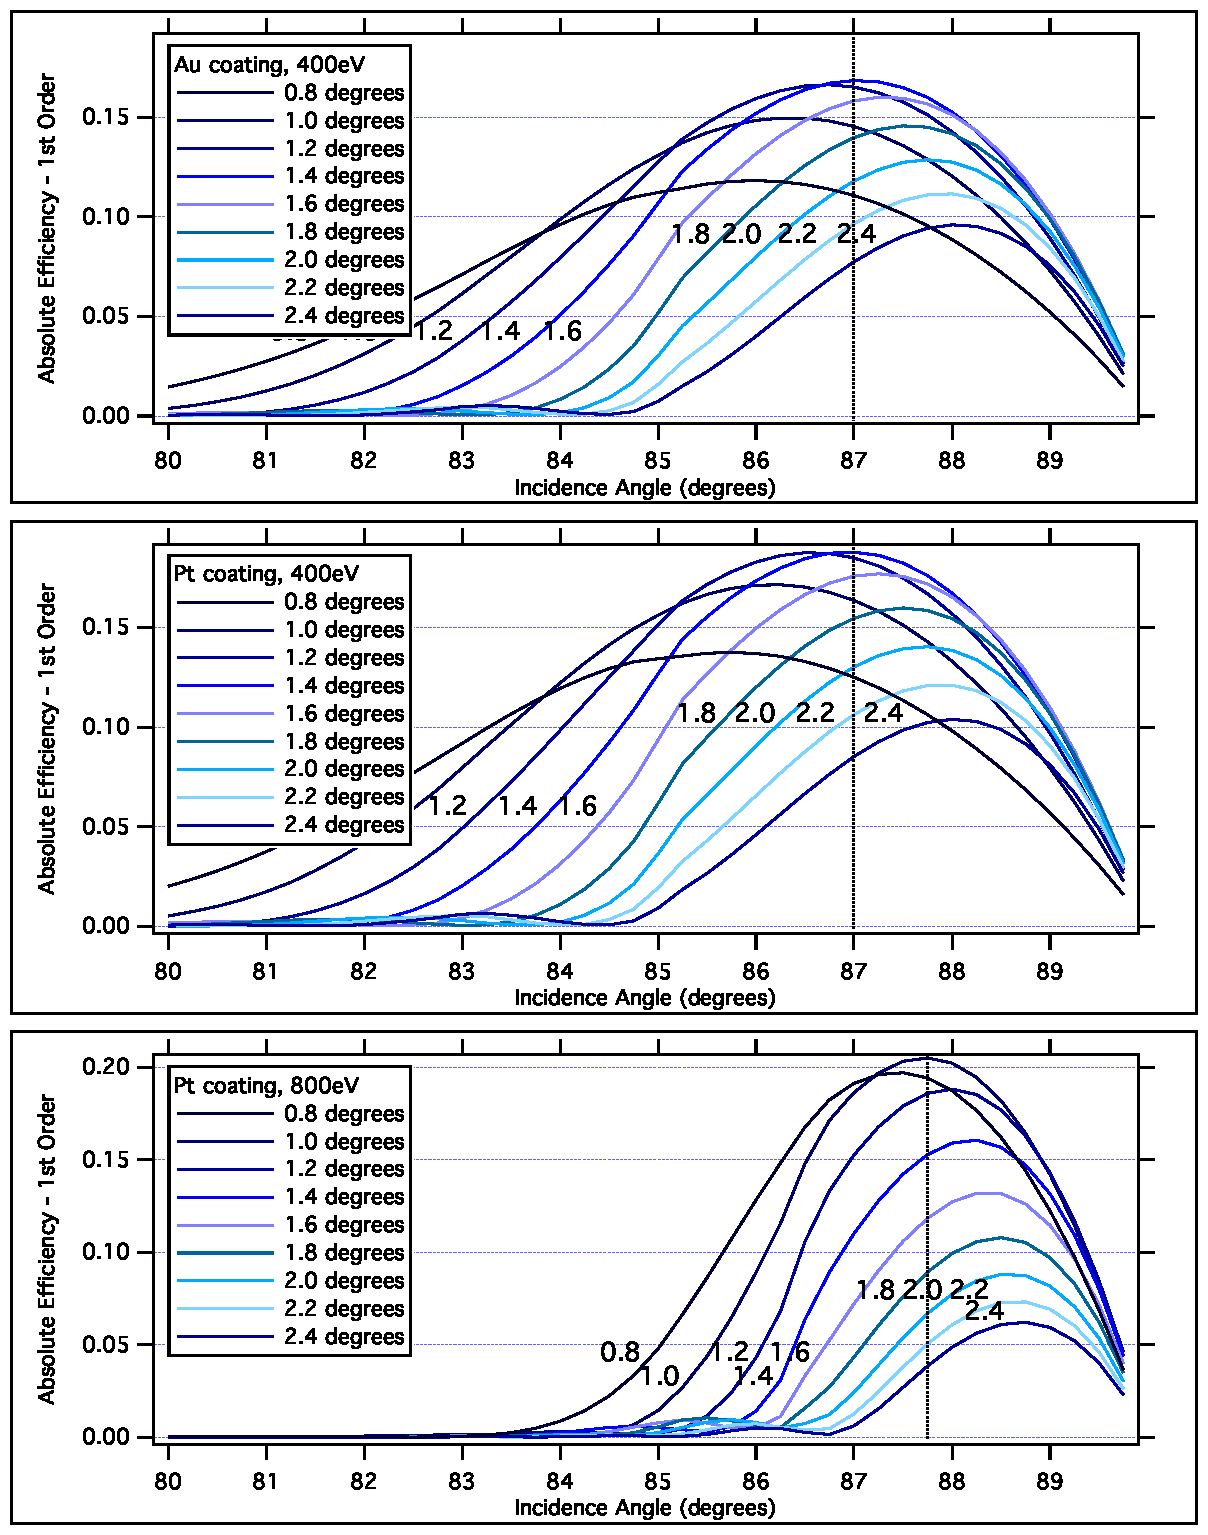
\includegraphics[width=\textwidth]{Chapter3/3i_incidenceAngle/3i_blazeChanges_solidColors.pdf} 
   \caption[While the blaze angle can always be used to tune a grating for a required incidence angle, there is still a particular \emph{optimal} incidence angle that -- when combined with a corresponding optimized blaze angle -- would produce the highest achievable efficiency.]{While the blaze angle can always be used to tune a grating for a required incidence angle, there is still a particular \emph{optimal} incidence angle that -- when combined with a corresponding optimized blaze angle -- would produce the highest achievable efficiency.  This optimal angle depends only on the groove density and energy.  (Gratings: all 1200 lines/mm; coatings, blaze angles, and energies as indicated.)}
   \label{3i-2}
\end{figure}

We found that the same effect happens for rectangular and sinusoidal gratings as well.  In each case, finding the optimal incidence requires a simultaneous optimization of the geometry parameters at each incidence angle tested: the blaze angle for triangular gratings, and the groove depth for rectangular and sinusoidal gratings.  (Because of the coupling between groove geometry and incidence angle, non-optimal geometry can otherwise hide the incidence maximum.)

Figure \ref{3i-2} contains an important take-away message for instrument designers: if an arbitrary incidence angle is required for some external reason, the geometry (blaze angle, depth, etc.) can be adjusted to optimize for that incidence. However, in the absence of constraints, there exists a unique optimal incidence angle (and corresponding groove geometry) where the efficiency reaches an absolute maximum.

Can we predict the optimal incidence analytically?  And does it actually only depend on the period and wavelength?  To answer these questions, we conducted a comprehensive search of the incidence angles that optimize first-order efficiency over a range of wavelengths and grating periods, for both blazed and rectangular gratings.  For every combination of wavelength and period, we needed to perform a global optimization of the incidence angle and groove geometry.\footnote{A global optimization was necessary particularly for the rectangular gratings, which exhibit periodic local maxima over the search space.}  We used the new \texttt{PEG} software, running massively in parallel on one of the Westgrid high-performance cluster computers, to conduct the optimization using a simple brute-force search over an adjustable parameter grid.\footnote{In the future, it would be desirable to add more sophisticated optimization methods to the software.}

\begin{figure}[htbp] %  figure placement: here, top, bottom, or page
   \centering
   \includegraphics[width=\textwidth]{Extended/OptimalIncidenceGlobalRect/results.pdf} 
   \caption[Optimizing the incidence angle and groove geometry for a range of wavelengths and grating periods shows a $n=-1$ order maximum at the $n=+1$ order Wood anomaly: $\sin \theta_{max} = 1 - \lambda/d$.]{Optimizing the incidence angle and groove geometry for a range of wavelengths and grating periods shows a $n=-1$ order maximum efficiency at angles described by $\sin \theta_{max} = 1 - \lambda/d$ [smooth curves].  This is the angle where the $n=+1$ order reaches $90\deg$: a Wood anomaly.  The optimization was conducted on a grid with an incidence step of 0.1\dg and a groove depth step of 0.002~um, using rectangular platinum gratings.}
   \label{rectIncidenceOpt}
\end{figure}

\subsection{Optimal incidence for rectangular gratings}
Figure \ref{rectIncidenceOpt} shows the optimal incidence angles found for rectangular gratings as a function of period and wavelength.  We discovered that we can accurately predict the optimal incidence angle $\theta_{max}$ according to the formula
\begin{align}
\label{rectOptimalIncidence}
\theta_{max} = \arcsin \left( 1 - \frac{\lambda}{d} \right),
\end{align}
plotted in the smooth curves for each period.  (Deviation from this formula and the optimized points is only due to the 0.1\dg precision of our optimization.)

There is a clear physical explanation for this result.  At grazing incidence, most of the outside ($n>0$) orders are evanescent, depending on the incidence angle.  If we assume an incidence angle so that an outside order $n'$ is propagating, and then we increase the incidence just to the point where it becomes evanescent, all of the energy previously carried by that wave will suddenly need to be re-distributed, increasing the efficiency of the remaining propagating orders.  The incidence angle where this happens occurs when the $n'$ outgoing angle reaches $90\deg$.  The effect is strongest in the case of the $n'=+1$ outside order; from the grating equation, we find:
\begin{align}
\sin \theta_{2,n'} &= \sin \theta_2 + n' \lambda / d \\
\sin \theta_{2,+1} &= \sin \theta_2 + \lambda / d\\
\sin (90\deg) &=  \sin \theta_2 + \lambda / d \\
\sin \theta_2 &= \sin \theta_{max} = 1 - \lambda/d
\end{align}

Therefore, the incidence angle for maximum inside first-order efficiency is the one that \emph{just} causes \emph{all} of the outside orders to be evanescent.  Historically, this has been referred to as a \emph{Wood anomaly of the Rayleigh type}, and it has been observed experimentally in visible light gratings as early as 1902 \cite{Woo02}.  Here, we show that we can predict it well using rigorous electromagnetic calculations via the differential method.

In visible light applications, Wood anomalies can be very sharp, and constitute a problem rather than an advantage by hiding or masking spectral lines; they can also be sensitive to polarization \cite{Ste62}.  In the grazing incidence soft x-ray domain, 
% TODO TODO IMPORTANT check this, add a plot?
 the efficiency increases and decreases smoothly on both sides of the peak; it does not drop off sharply even when the $+1$ order is actually propagating, but still close to 90\dg.  (We also confirmed using \texttt{Gradif} that it is insensitive to polarization.)  Therefore, we actually suggest \emph{exploiting} the $+1$ Wood anomaly as a starting point when designing constant-incidence x-ray instruments.  For photon energies above 100 eV, the peak width should provide a usable instrumental range, but designers should always check the efficiency spectrum over wavelength to ensure that it is wide enough for their range of interest.  At low photon energies, an incidence angle slightly higher than $\theta_{max}$ can widen the range with only a small decrease in the peak efficiency.

\subsection{Optimal incidence for blazed gratings}
From these results, we would also expect to find the optimal incidence for blazed gratings at the $+1$ Wood anomaly.  However, the actual optimal incidence angle turns out to significantly more grazing than predicted by Equation \eq{rectOptimalIncidence}; the results are shown in Figure \ref{blazedIncidenceOpt}.  The difference is significant: in some cases we have observed a doubling in the efficiency from the angle predicted in Equation \eq{rectOptimalIncidence} and the true optimal incidence.  The explanation for the difference is related to the blazing effect, but we have not yet discovered an analytic formula to predict it. So far, it must be determined via optimization.

\begin{figure}[htbp] %  figure placement: here, top, bottom, or page
   \centering
   \includegraphics[width=\textwidth]{Extended/OptimalIncidenceGlobalBlazed/round2/results.pdf} 
   \caption[Unlike rectangular gratings, the optimal incidence angle for blazed gratings (marked points) does not follow the curve for the +1 order Wood Anomaly (dashed lines).]{Unlike the case of rectangular gratings, the optimal incidence angles for blazed gratings (marked points) do not follow the curves for the +1 order Wood Anomalies (dashed lines).  Instead, the optimal incidence needs to be determined through optimization.}
   \label{blazedIncidenceOpt}
\end{figure}


% TODO: calculations to highlight how important/effective this is.  Efficiency at non-optimal and optimal incidence, when optimizing geometry.
% TODO: polarization dependence

\section{Effect of anti-blaze angle for blazed gratings}
Blazed gratings are reported to be most efficient with a perfect anti-blaze angle of 90\dg \cite{Pal05}.  When ordering gratings from a manufacturer, the tolerance for the anti-blaze angle must be specified.  In Figure \ref{3k}, we calculate the effect of the anti-blaze angle on the efficiency spectrum.  For grazing-incidence optics, it turns out that as long as the anti-blaze angle is greater than approximately eight times the blaze angle, it has almost no effect on the efficiency.

\begin{figure}[htbp] %  figure placement: here, top, bottom, or page
   \centering
   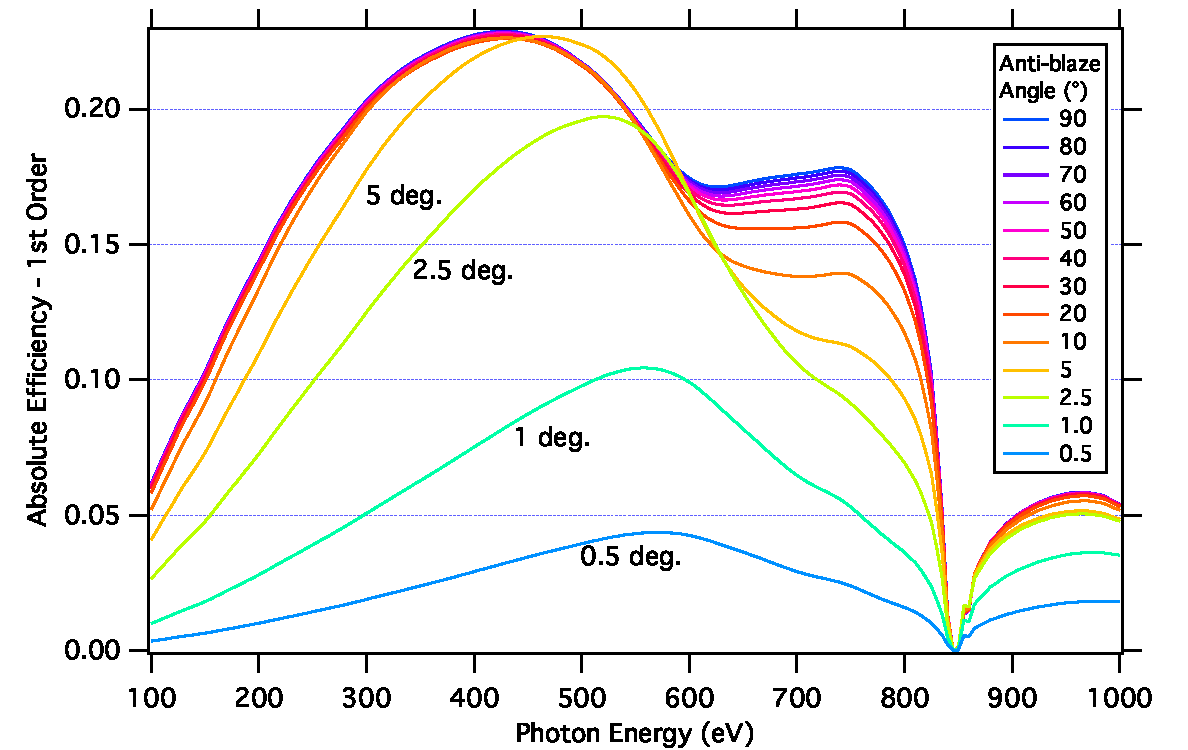
\includegraphics[width=\textwidth]{Chapter3/3k_antiBlazeAngle/3k.pdf} 
   \caption[These calculations over a range of anti-blaze angles show that as long as the anti-blaze angle is greater than $\sim$4 times the blaze angle, it has almost no effect on the efficiency.]{These calculations over a range of anti-blaze angles show that as long as the anti-blaze angle is greater than $\sim$8 times the blaze angle, it has almost no effect on the efficiency.  (Grating: 1200~lines/mm; Nickel coating; 88\dg incidence; 1.48\dg blaze angle.)}
   \label{3k}
\end{figure}
	
\section{Applications to beamline and instrument design}
Beamline designers can use the observations in this chapter to guide the design process.  Starting with the choice of the groove shape, it is clear that blazed profiles will always offer the best performance for constant-incidence applications like the spectrometer in Chapter 6.  For variable-incidence designs like monochromators, a blazed profile optimized for the centre of the instrument's wavelength range will lose efficiency at the extremes, but might still offer better performance than a sinusoidal grating, especially if the total range is being divided across multiple gratings. (This can be verified quickly using the constant-included-angle scan in the \texttt{PEG} software.)

Next, a groove density should be chosen that is as low as possible while still providing the required resolution.  In the next chapter, we explore a novel way of increasing resolution while maintaining a moderate groove density.

For constant-incidence instruments, designers should consider using the optimal angle discovered in Section \ref{incidenceAngle}.  For rectangular gratings Equation \eq{rectOptimalIncidence} can be used. At low photon energies ($<100$ eV), the width of the anomaly's efficiency peak might not be sufficient to cover the desired energy range; using a slightly more grazing incidence angle and re-optimizing the groove geometry tends to widen the peak with an acceptable reduction in the maximum efficiency.
% TODO: check this with a plot.
For blazed gratings, the optimal incidence should be found through an optimization at the design wavelength and period.  

\textbf{Warning:} We should also note here that in most instrument configurations, a lower (more normal) incidence creates a larger acceptance angle for the grating and therefore increases the \emph{geometric} efficiency. The change in the diffraction efficiency as a result of the incidence angle should always be evaluated in conjunction with the change in geometric efficiency.
%  (As a practical example, we applied this technique in the design of the REIXS spectrometer in Chapter 6; it explains why the incidence angles for the low groove density gratings are more normal than the high groove density gratings.)

When choosing a blaze angle, designers should keep in mind that the bandwidth of the blazed efficiency peak increases both with photon energy and groove density: optimizing for low energies near 100 eV creates narrow efficiency peaks; at higher energies, the peaks become wider and the gratings can be more general.
% TODO plot to show this?
Figure \ref{3e-2} shows the same increase in generality as a function of groove density.

Finally, our calculations for the effect of the anti-blaze angle (Figure \ref{3k}) show that the tolerance specified for this parameter can be quite large; instead, grating manufacturers should concentrate on achieving a very accurate blaze angle.

\section{Validation: comparison of theory to experimental results}
We have provided these recommendations to beamline designers based on a purely theoretical survey of the factors affecting grating efficiency.  For these results to be trustworthy, we need to confirm that the theory in Chapter 3 and the implementations in Chapter 4 are accurate descriptions of the real world.  (We move on in Chapter 6 to use these tools to design the gratings and  layout for the REIXS beamline spectrometer; before starting that project, we needed our own confirmation of the software's accuracy.)

The published literature on soft x-ray gratings includes only a few measurements of real-world efficiency.  This is partly due to the difficulty of completing these measurements, and partly because, after receiving brand new gratings, most beamline builders would rather install them as quickly as possible and start doing their own research, rather than spend time on another beamline characterizing the gratings.  This is unfortunate for two reasons.  Beamline scientists often do not know the efficiency of their machines, or even whether the gratings they have received are optimal. Additionally, grating theorists do not have a large set of experimental results for validating their calculation methods in the soft x-ray regime.

 We found one study by M. Bowler at the SRS light source \cite{Bow01} with a recent set of efficiency measurements for four gratings representing three different types of grating profiles.  The gratings include one blazed grating with 1440 lines/mm, one rectangular grating with 600 lines/mm, and two attempted-rectangular gratings that ended up with trapezoidal sides of approximately $57\deg$.  The geometry parameters of all of the gratings were well-characterized by the manufacturer after ruling, making them ideal for comparing to theory.  (The study also conducted efficiency calculations using the differential method, but we duplicated these calculations as a double-check on our implementations.)

Figures \ref{3j-1} through \ref{3j-4} show these experimental measurements, combined with our own calculations of the grating efficiency.  Table \ref{3j-table} provides the geometry parameters, derived from the manufacturer's measurements.

\begin{table}[htbp]
\centering
\topcaption[Geometry parameters and incidence configuration for the gratings in Figures \ref{3j-1} to \ref{3j-4}.]{Geometry parameters and incidence configuration for the gratings in Figures \ref{3j-1} to \ref{3j-4}.  The geometry measurements were taken at the centre of the grating; accurate characterization of these gratings after ruling made them ideal for comparing with theoretical calculations. CIA stands for ``constant included angle'' -- a mounting configuration that maintains a constant angle between the incident direction and 1st order.}
{\footnotesize
\begin{tabularx}{\textwidth}{@{} l c l r @{}} % Column formatting, @{} suppresses leading/trailing space
\toprule
Profile    &  Density (lines/mm)& Geometry Parameters & CIA ($\deg$)\\
\midrule
Blazed & 1440 & Blaze angle: 2.2$\deg$, anti-blaze: 12.8$\deg$ & 160 \\
Rectangular & 600 & Depth: 22.2 nm, valley width: 1.12 um & 167 \\
Trapezoidal & 300 & Depth: 49.3 nm, valley width: 2.46 um, angle: 57$\deg$ & 167\\
Trapezoidal & 390 & Depth: 54.0 nm, valley width: 1.39 um, angle: 57$\deg$ & 160\\
\bottomrule
\end{tabularx}
}
\label{3j-table}
\end{table}

\subsection{Note on incidence angle}
Unlike the constant incidence angle efficiency curves we have been using up to this point, these gratings were designed for use in constant-included-angle monochromators, where the included angle $(\theta_2 + \theta_{2,n})$ between the incident beam and the useful order $n$ is held constant.  
Therefore, these plots show the efficiency as a function of energy, with an incidence angle that also varies along the $x$-axis according to this constraint.

\subsection{Comparison to theory}
Of particular interest are the 1st and 2nd order results for the blazed grating in Figure \ref{3j-1}, since we settled on blazed gratings for the design in Chapter 6.  The agreement in the shape and amplitude of the efficiency spectra is very good; we can expect that the real-world efficiency would be slightly lower than predicted due to surface roughness and other effects described in Section \ref{realWorldEffects}.  The agreement for the laminar profile in Figure \ref{3j-2} is also very good.  Figures \ref{3j-3} and \ref{3j-4} show a tendency for the calculated results on the trapezoidal gratings to be shifted toward lower energies with respect to the measurements, although the shift is less than 20 eV.  Overall, the close agreement between the theoretical and measured efficiencies shown here gives us a high degree of confidence in applying the grating software to optimize real-world beamlines.
 
 % Previously: all width=\textwidth were scale=0.78
\begin{figure}[htbp] %  figure placement: here, top, bottom, or page
   \centering
   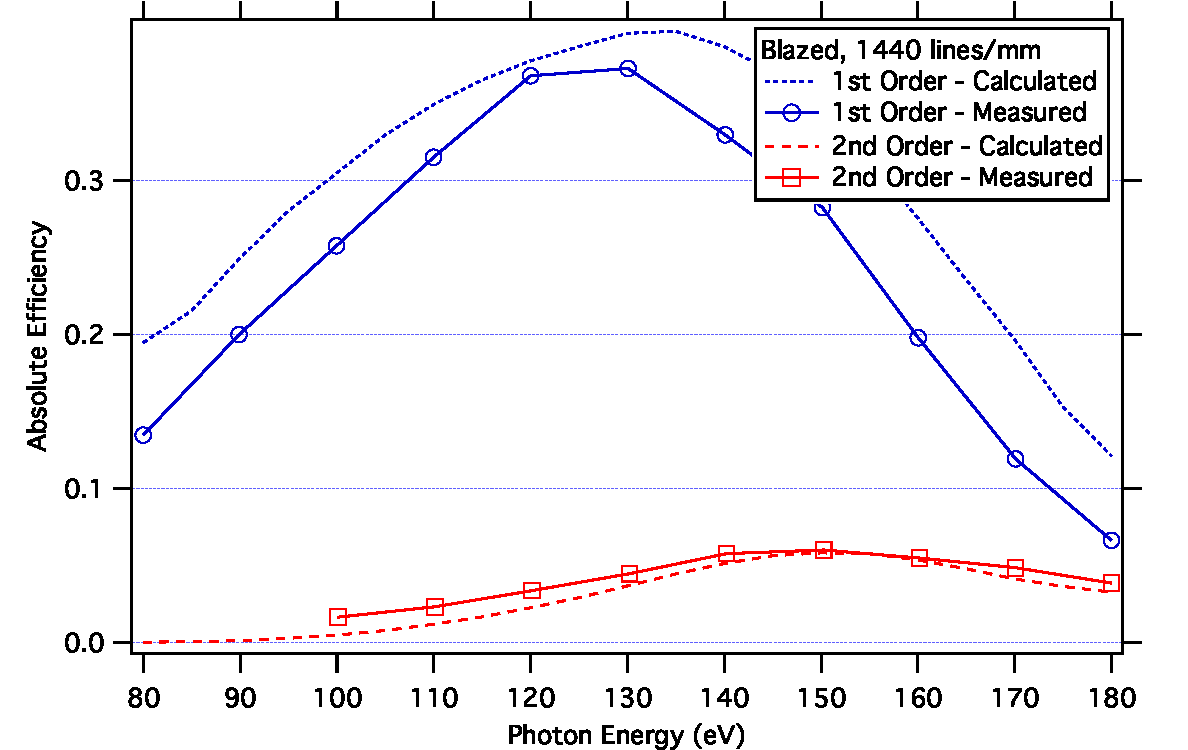
\includegraphics[width=\textwidth]{Chapter3/3j_comparisonWithExperimental/3j_blazed.pdf} 
   \caption{Comparison of grating efficiency calculations to diffractometer measurements.  Blazed grating, 1440 lines/mm, 2.2$\deg$ blaze angle, 12.8$\deg$ anti-blaze angle. Incidence: 160$\deg$ constant included angle to the 1st inside order.}
   \label{3j-1}
\end{figure}

\begin{figure}[htbp] %  figure placement: here, top, bottom, or page
   \centering
   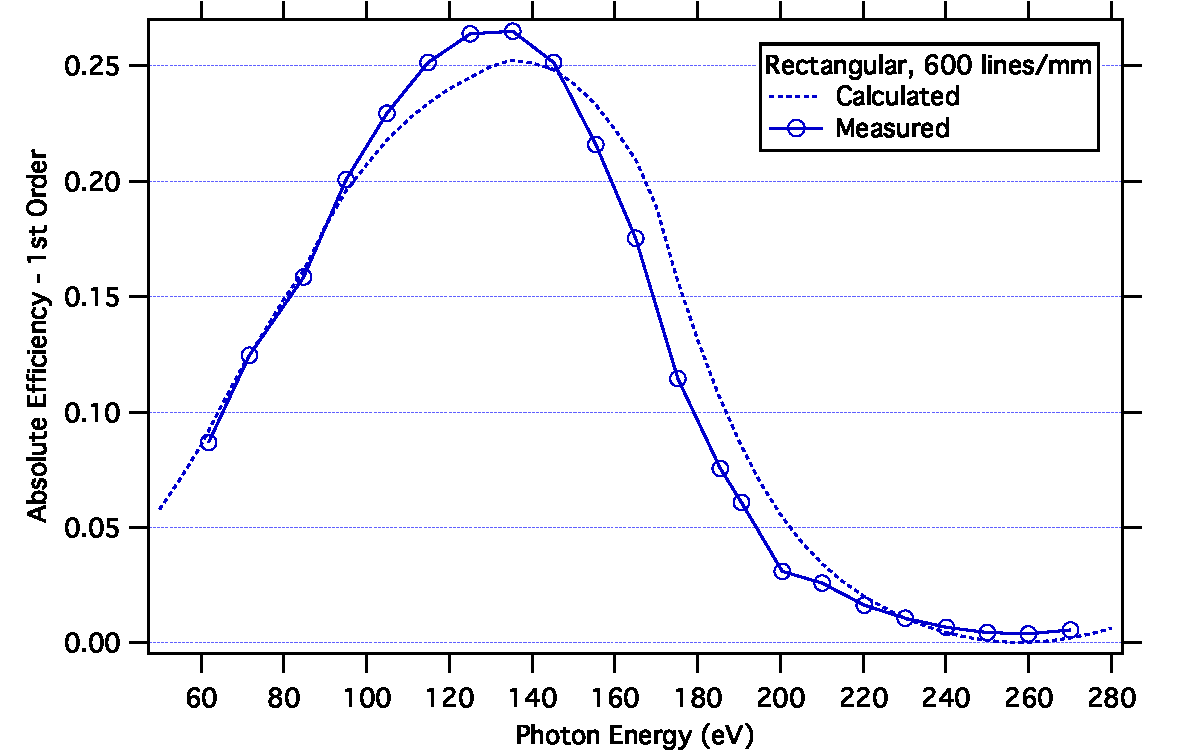
\includegraphics[width=\textwidth]{Chapter3/3j_comparisonWithExperimental/3j_laminar.pdf} 
   \caption{Comparison of grating efficiency calculations to diffractometer measurements.  Rectangular grating, 600 lines/mm, 22.2 nm depth, 1.12 um valley width.  Incidence: 167$\deg$ constant included angle to the 1st inside order.}
   \label{3j-2}
\end{figure}

\begin{figure}[htbp] %  figure placement: here, top, bottom, or page
   \centering
   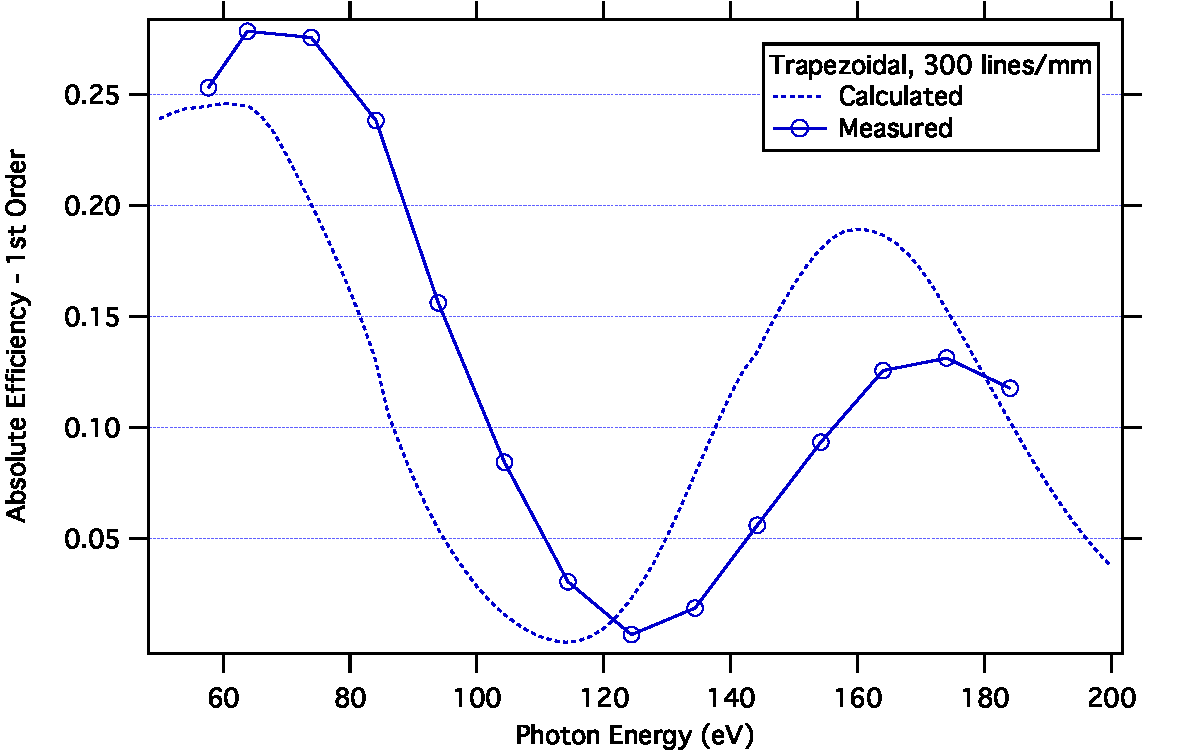
\includegraphics[width=\textwidth]{Chapter3/3j_comparisonWithExperimental/3j_trap300.pdf} 
   \caption{Comparison of grating efficiency calculations to diffractometer measurements.  Trapezoidal grating, 300 lines/mm, 57$\deg$ side angles, 49.3 nm depth, 2.46 um valley width.  Incidence: 167$\deg$ constant included angle to the 1st inside order.}
   \label{3j-3}
\end{figure}

\begin{figure}[htbp] %  figure placement: here, top, bottom, or page
   \centering
   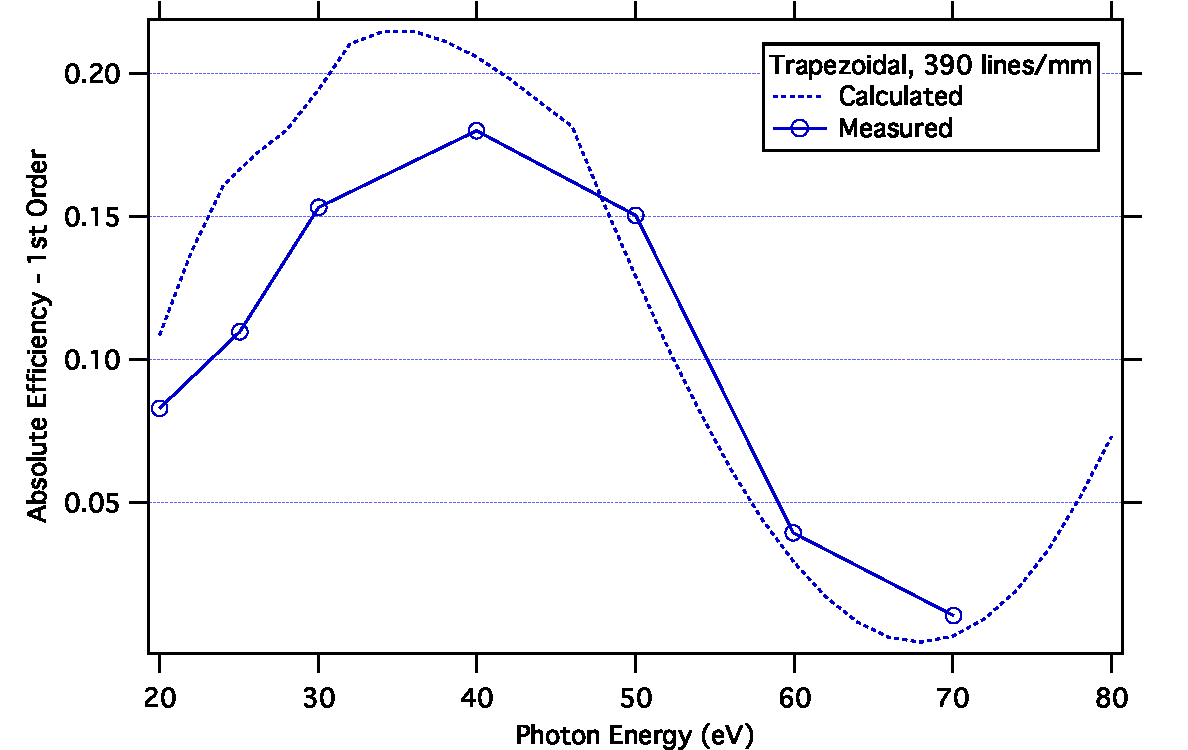
\includegraphics[width=\textwidth]{Chapter3/3j_comparisonWithExperimental/3j_trap390.pdf} 
   \caption{Comparison of grating efficiency calculations to diffractometer measurements.  Trapezoidal grating, 390 lines/mm, 57$\deg$ side angles, 54 nm depth, 1.39 um valley width.  Incidence: 160$\deg$ constant included angle to the 1st inside order.}
   \label{3j-4}
\end{figure}
